\documentclass{puthesis-UG}

\usepackage{style}

%%%%%%%%IMPORTANT INFORMATION%%%%%%%%%%%%%%%%%%%%
%Using puthesis-UG.cls includes an Honor Code declaration. By using this file you are 
%declaring that this paper is your own work in accordance with University retgulations.
%
%The file puthesis-UG.cls must be downloaded from the math department website and 
%saved in the same directory as this file.
%%%%%%%%%%%%%%%%%%%%%%%%%%%%%%%%%%%%%%%%

\author{Alan Yan}
\adviser{Professor June E. Huh}
\title{Hodge-Riemann Relations of the Basis Generating Polynomial of a Matroid}
\abstract{(write something flowery)}
\acknowledgements{I would like to thank}
\date{today}


% Things I want to talk about:

% 1. Combinatorial Atlas
% 2. Lorentzian Polynomials
% 3. Alexandrov-Fenchel Inequality
% 4. 
%


\begin{document}
 
\chapter{Conventions and Notation}

\chapter{Introduction}

\chapter{Combinatorial Structures}

\section{Partially Ordered Sets}

Our main reference for partially ordered sets is \cite{ordered-sets}. 
\begin{defn}
	A \textbf{partially ordered set} is an ordered pair $(P, \leq)$ of a set $P$ and a binary relation $\leq$ on $P$ such that 
	\begin{enumerate}
		\item[(\textbf{P1})] $x \leq x$ for all $x \in P$. 
		\item[(\textbf{P2})] If $x \leq y$ and $y \leq x$, then $x = y$. 
		\item[(\textbf{P3})] If $x \leq y$ and $y \leq z$, then $x \leq z$. 
	\end{enumerate}
\end{defn}

\begin{example}
	We provide a list of exmaples of common posets which appear naturally in mathematics. 
	\begin{enumerate}[label = (\alph*)]
		\item Any subset of the real numbers equipped with the less-than-or-equal-to relations $\leq$.
		\item Any subset of the integers equipped with the divisibility relation.
		\item Any collection of sets equipped with the inclusion relation. 
		\item The vertices of a directed graph where $v \leq w$ if and only if $w$ can be reached from a directed path started at $v$. 
	\end{enumerate}
\end{example}

\subsection{Linear Extensions}

\begin{defn}
	Let $(P, \leq)$ be a poset on $n$ elements. A \textbf{linear extension} is any bijective map $f : P \to [n]$ satisfying $f(x) < f(y)$ for all $x, y \in P$ satisfying $x < y$.
\end{defn}
\subsection{Lattices}

\begin{defn}
	We say a poset $\mcL$ is a lattice if for any $x, y \in \mcL$ there exist (unique) poset elemenets $x \vee y$ (called the \textbf{meet} or \textbf{greatest lower bound}) and $x \wedge y$ (called the \textbf{join} or \textbf{least upper bound}) satisfying 
	\begin{enumerate}
		\item[(\textbf{L1})] $x \vee y \geq x$, $x \vee y \geq y$, and for any $z \in \mcL$ satisfying $z \geq x$ and $z \geq y$, we have $z \geq x \vee y$. 
		\item[(\textbf{L2})] $x \wedge y \leq x$, $x \wedge y \leq y$, and for any $z \in \mcL$ satisfying $z \leq x$ and $z \leq y$, we have $z \leq x \wedge y$. 
	\end{enumerate}
\end{defn}

The only lattice that we will be concerned with are geometric lattices. 
\section{Graph Theory}

We assume a working knowledge of basic graph theory. This includes concepts such as connected components, paths, trees, etcetera. We provide the definition of a graph that we will use in this paper. Note that we allow multi-edges and but not loops. This is because in later results concerning graphic matroids, the presense of loops does not affect log-concavity. Our main reference for basic notions in graph theory come from \cite{diestel}. For more the more sophistication notions that come from spectral graph theory, we refer to \cite{chung-spectral-graph-theory}. 

\begin{defn}
	A \textbf{graph} is an ordered pair $(V, E)$ of vertices and edges such that each edge is associated with either two distinct vertices or one vertex. If an edge is associated with two distinct vertices, then we call it a \textbf{simple edge}. If an edge is associated with one vertex, then we call it a \textbf{loop}. 
\end{defn}

\subsection{Spectral Graph Theory}

\begin{defn}
	Given a graph $G$ with $n$ vertices $v_1, \ldots, v_n$, we define its Laplacian matrix $L := L_G$ to be the $n \times n$ matrix defined element-wise as 
	\[
		L_{i, j} := \begin{cases}
			\deg (v_i) & \text{if $i = j$} \\
			-E_{v_i, v_j} & \text{if $i \neq j$ and $v_i$ is adjacent to $v_j$}
		\end{cases}
	\]
	where $E_{v_i, v_j}$ is the number of edges between $v_i$ and $v_j$. 
\end{defn}

\begin{defn}
	Let $G$ be a graph and let $V = \{v_1, \ldots, v_n\}$ be an arbitrary ordering of the vertices. For this ordering, we can define a $|V| \times |E|$ matroid $B_G$ called the \textbf{incidence matrix} where the entry indexed by $v \in V$ and $e = \{v_i, v_j\} \in E$ where $v_i > v_j$ is equal to 
	\[
		B_{ve} = \begin{cases}
			1, & \text{if $v = v_i$} \\
			-1, & \text{if $v = v_j$} \\
			0, & \text{otherwise.}
		\end{cases}
	\]
	The matrix $C_G$ which is obtained by removing the last row of $B_G$ is called the \textbf{reduced incidence matrix}. 
\end{defn}

The incidence matrix and reduced incidence matrix satisfy the condition in Proposition~\ref{incidence-reduced-incidence-matrix-is-good}. This connects the linear independence of the columns of the incidence matrices of $G$ to the cyclelessness of subgraphs of $G$. This proposition will provide an example of the combinatorial structure of a matroid introduced in the subsequent section. 

\begin{prop} \label{incidence-reduced-incidence-matrix-is-good}
	For a graph $G = (V, E)$ the incidence matrix $B_G$ and reduced incidence matrix $C_G$ both satisfy the property that a set of columns are linearly independent if and only if the graph formed by the corresponding edges does not contain a cycle. 
\end{prop}

\begin{proof}
	See Example 5.4 of \cite{bapat_raghavan_1997}. 
\end{proof}


\section{Matroids}

Matroids can be thought of as combinatorial objects which abstracts and generalizes the properties of both linear independence in vectors spaces and cyclelessness in graphs. Despite the seemingly limited scope of this interpretation, matroids successfully describe many objects relevant to other areas in mathematics such as topology \cite{gelfand}, graph theory \cite{milnor-numbers}, combinatorial optimization \cite{optimization}, algebraic geometry \cite{schubert-cell}, and convex geometry \cite{matroid-polytope}. In this subsection, we provide an introduction to the basic notions in matroid theory that we will need in the remainder of this thesis. We use the excellent monographs \cite{10.5555/1197093} and \cite{welsh} as our main references for the basic theory.

\subsection{Independent Sets}
\begin{defn}
	A \textbf{matroid} is an ordered pair $M = (E, \mcI)$ consisting of a finite set $E$ and a collection of subsets $\mathcal{I} \subseteq 2^E$ which satisfy the following three properties:
	\begin{enumerate}
		\item[(\textbf{I1})] $\emptyset \in \mathcal{I}$. \footnote{(\textbf{I1}) is the \textbf{non-emptiness} axiom}
		\item[(\textbf{I2})] If $X \subseteq Y$ and $Y \in \mathcal{I}$, then $X \in \mathcal{I}$.\footnote{(\textbf{I2}) is the \textbf{hereditary} axiom}
		\item[(\textbf{I3})] If $X, Y \in \mathcal{I}$ and $|X| > |Y|$, then there exists some element $e \in X \backslash Y$ such that $Y \cup \{e\} \in \mathcal{I}$. \footnote{(\textbf{I3}) is the \textbf{exchange} axiom}
	\end{enumerate}
	The set $E$ is called the ground set of the matroid and the collection of subsets $\mathcal{I}$ are called independent sets. This naming convention is motivated by Example~\ref{linear-matroid} where the indepedent sets consist exactly of sets of linearly independent vectors. 
\end{defn}

\begin{example} [Linear Matroids] \label{linear-matroid}
	Let $V$ be a $k$-vector space and let $E = \{v_1, \ldots, v_n\}$ be a finite set of vectors from $V$. If we let $\mcI$ consist of all subsets of $E$ which are linearly independent, then $(E, \mcI)$ forms a matroid. We call any matroid which can be constructed in this way a \textbf{linear matroid}. 
\end{example}

\begin{example} [Graphic Matroids]
	Let $G = (V, E)$ be a graph and let $\mcI$ be the collection of subsets of $E$ which consist of edges containing no cycles. Then $(E, \mcI)$ forms a matroid called the \textbf{cycle matroid} of the graph $G$. We call any matroid which is isomorphic to a cycle matroid of a graph a \textbf{graphic matroid}. In Proposition~\ref{graphic-are-linear}, we prove that graphic matroids are not only linear, but they can be represented by a totally unimodular matrix. 
\end{example}

\begin{prop} \label{graphic-are-linear}
	
\end{prop}

Given a matroid $M = (E, \mathcal{I})$, we call a subset $X \subseteq E$ a \textbf{dependent set} if and only if $X \notin \mathcal{I}$. Given a matroid, we call any minimal dependent set a \textbf{circuit}. Matroids are uniquely determined by their circuits. For a proof of this fact, see Corollary 1.1.5 in \cite{10.5555/1197093}.

\subsection{Bases}
We define a basis $B \in \mathcal{I}$ to be a maximal independent set. From property (\textbf{I3}), we can deduce that all bases have the same number of elements. Indeed, if $B_1$ and $B_2$ are bases satisfying $|B_1| < |B_2|$ then from (\textbf{I3}) there exists some element $e \in B_2 \backslash B_1$ satisfying $B_1 \cup \{e\} \in \mcI$. But, this means that $B_1 \cup \{e\}$ is an independent set strictly larger than $B_1$. This contradicts the maximality of $B_1$ and implies that all bases contain the same number of elements. 
\begin{defn}
	Let $M = (E, \mathcal{I})$ be a matroid and let $\mcB$ be the collection of bases. Then, the following three properties (Lemma 1.2.2 in \cite{10.5555/1197093}):
	\begin{enumerate}
		\item[\textbf{(B1)}] $\mcB$ is non-empty.
		\item[\textbf{(B2)}] If $B_1$ and $B_2$ are members of $\mcB$ and $x \in B_1 \backslash B_2$, then there is an element $y$ of $B_2 \backslash B_1$ such that $(B_1 - x) \cup y \in \mcB$. 
		\item[\textbf{(B3)}] If $B_1$ and $B_2$ are members of $\mcB$ and $x \in B_1 \backslash B_2$, then there is an element of $y \in B_2 \backslash B_1$ such that $(B_2 - y) \cup x \in \mcB$. 
	\end{enumerate}
\end{defn}

Associated with the bases of a matroid, we can define the \textbf{basis generating function} of a matroid $M = (E, \mcB)$ as
\[
	f_M (x) := \prod_{B \in \mcB} x^B \in \RR[x_e : e \in E]
\]
which is a homomogeneous polynomial in the ring of polynomials with variables indexed by the ground set of our matroid. 

\subsection{Rank Functions}

\begin{defn}
	For any matroid $M = (E, \mcI)$, we define its rank function $\rank_M : 2^E \to \NN$ to be equal to
	\[
		\rank_M(X) := \max \{|I| : I \in \mathcal{I}, I \subseteq X\}.
	\]
	The rank function satisfies the following three properties (Lemma 1.3.1 in \cite{10.5555/1197093}):
	\begin{enumerate}
		\item[(\textbf{R1})] If $X \subseteq E$, then $0 \leq r(X) \leq |X|$. 
		\item[(\textbf{R2})] If $X \subseteq Y \subseteq E$, then $r(X) \leq r(Y)$. 
		\item[(\textbf{R3})] If $X$ and $Y$ are subsets of $E$, then $r(X \cup Y) + r(X \cap Y) \leq r(X) + r(Y)$.
	\end{enumerate}
\end{defn}


\subsection{Closure Operators and Lattice of Flats}

\begin{defn}
	For any matroid $M = (E, \mcI)$, we define its closure operator $\clo_M : 2^E \to 2^E$ to be 
	\[
		\clo_M (X) := \overline{X} = \{x \in E : \rank (X \cup \{x\}) = \rank (X) \}.
	\]
	The closure operator satisfies the following four properties (Lemma 1.4.3 in \cite{10.5555/1197093}):
	\begin{enumerate}
		\item[(\textbf{C1})] If $X \subseteq E$, then $X \subseteq \clo_M (X)$. 
		\item[(\textbf{C2})] If $X \subseteq Y \subseteq E$, then $\clo_M (X) \subseteq \clo_M (Y)$. 
		\item[(\textbf{C3})] If $X \subseteq E$, then $\clo_M (\clo_M(X)) = \clo_M(X)$. 
		\item[(\textbf{C4})] If $X \subseteq E$ and $x \in E$, and $y \in \clo_M(X \cup \{x\}) \backslash \clo_M(X)$, then $x \in \clo_M(X \cup \{y\})$. 
	\end{enumerate}
\end{defn}

\begin{example}
	Let $M := M(\{v_1, \ldots, v_n\})$ be the linear matroid represented by vectors $v_1, \ldots, v_n$ in a $k$-vector space $V$. Then, the closure of a subset $X \subseteq \{v_1, \ldots, v_n\}$ is precisely $\clo_M(X) := \{v_1, \ldots, v_n\} \cap \mathsf{span}_k X$. 
\end{example}

If $X \subseteq E$ satisfies $X = \clo_M(X)$, then we say $X$ is a \textbf{closed set} or \textbf{flat}. For any matroid $M = (E, \mcI)$, let $\mcL(M)$ denote the partially ordered set consisting of the flats of $M$ equipped with set inclusion. 

\begin{prop}[Theorem 1.7.5 in \cite{10.5555/1197093}]
	Let $M = (E, \mcI)$ be a matroid. Then, the poset $\mcL(M)$ is a geometric lattice with join and meet operations defined as $X \vee Y := \clo_M(X \cup Y)$, $X \wedge Y := X \cap Y$, and rank function $\rank_{\mcL} (X) := \rank_M(X)$. 
\end{prop}


\subsection{Loops and Parallel Elements}
We say $e \in E$ is a \textbf{loop} in $M$ if $\{e\}$ is a dependent set. Equivalently, $e \in E$ is a loop if $\rank (\{e\}) = 0$. We define $E_0$ as the set of loops. An element $e \in E$ in the ground set is called a \textbf{coloop} if it is contained in every basis. We say $x_1, x_2 \in E \backslash E_0$ satisfy $x_1 \sim_M x_2$ if and only if $\{x_1, x_2\} \notin \mcI$ or $x_1 = x_2$. Equivalently, $x_1 \sim_M x_2$ if and only if $\rank (\{x_1, x_2\}) = 1$. When $x_1 \sim_M x_2$, we say that $x_1$ and $x_2$ are \textbf{parallel}. For a more in-depth treatment of loops and parallelism, I refer the reader to section 1.4 of \cite{welsh}.

\begin{prop} \label{parallelism-is-equivalence-relation}
	Let $M = (E, \mcI)$ be a matroid. Then $\sim_M$ is an equivalence relation on $E \backslash E_0$. 
\end{prop}

\begin{proof}
	For any $x \in E \backslash E_0$, we have $\rank (\{x, x\}) = \rank (\{x\}) = 1$ since $x \notin E_0$. Thus $x \sim_M x$. For $x, y \in E \backslash E_0$, we have $\rank (\{x, y\}) = \rank \{y, x\}$. This proves that $\sim_M$ is reflexive. To prove transitivity, suppose that we have $x, y, z \in E$ that satisfy $x \sim_M y$ and $y \sim_M z$. If $x = y$ or $y = z$, then we automatically get $x \sim_M z$. Suppose that they are all distinct. Then, we have $\{x, y\}, \{y, z\} \not\in \mcI$. For the sake of contradiction, suppose that $\{x, z\} \in \mcI$. From (\textbf{I3}) applied to $\{x, z\}$ and $\{y\}$, we have that either $\{x, y\} \in \mcI$ or $\{y, z\} \in \mcI$. This is a contradiction. This proves that $\sim_M$ is transitive and an equivalence relation. 
\end{proof}

From Proposition~\ref{parallelism-is-equivalence-relation}, for any non-loop $e \in E \backslash E_0$, we can consider its equivalence class $[e] := [e]_M$ under the equivalence relation $\sim_M$. We call the equivalence class $[e]$ the \textbf{parallel class} of $e$. Then, we can partition the ground set $E$ into $E = E_1 \sqcup E_2 \sqcup \ldots \sqcup E_s \sqcup E_0$ where $E_1, \ldots, E_s$ are the distinct parallel classes and $E_0$ are the loops. In Proposition~\ref{characterization-of-atoms-of-flats}, we give a characterization of the atoms of the lattice of flats in terms of the parallel classes and loops. 

\begin{prop} \label{characterization-of-atoms-of-flats}
	Let $M = (E, \mcI)$ be a matroid and let $e \in E$ be an element of the matroid that is not a loop. Then, $\overline{e} = [e] \cup E_0$.
\end{prop}

\begin{proof}
	Since any independent set contains no loops, we know that $E_0 \subseteq \overline{e}$. For any $f \in [e]$, we have that $\rank (\{e, f\}) = 1 = \rank (\{e\})$ by definition of $\sim_M$. This proves that $[e] \subseteq \overline{e}$. To prove the opposite inclusion, let $f \in \overline{e}$. Then $\rank(\{e, f\}) = 1$. If $f$ is a loop, then $f \in E_0$. Otherwise, $f \sim_M e$ and $f \in [e]$. This suffices for the proof of the proposition. 
\end{proof}

We call a matroid $\textbf{simple}$ if it contains no loops and no parallel elements. To every matroid $M$, we can associate a simple matroid $\widetilde{M}$ called the \textbf{simplification} of the matroid $M$. For any matroid $M = (E, \mcI)$, let $\pi_M : E \to 2^E$ be the map $\pi_M (e) = \overline{e}$ which sends a matroid element to its closure. When $e$ is not a loop, then $\overline{e}$ is a one-dimensional flat. If $e$ is a loop, then $\overline{e} = E_0$. From Proposition~\ref{characterization-of-atoms-of-flats}, we can think of $\pi_M (E)$ as the set of one-dimensional flats and the set of loops. 

\subsection{Contraction and Deletion}

In graph theory, there are notions of edge contraction and edge deletion. In Definition, we genealize contraction and deletion from graphs to general matroids. When applying contraction and deletion in the matroid sense to graphic matroids, we recover edge contraction and deletion in graph theory.  

\begin{defn}[Restriction, Contraction, and Deletion]\label{contraction-deletion}
	Let $M = (E, \mcI)$ be a matroid and let $T \subseteq E$ be a subset. We define $M|_T$ to be the restriction of $M$ on $T$ as the matroid on $T$ with independent sets 
	\[
		\mcI (M|_T) := \{I \in \mcI : I \subseteq T\}.
	\]
	The deletion $M \backslash T$ of $T$ from $M$ is then defined to be the restriction $M|_{E \backslash T}$. Let $B_T$ be a basis of $M|_T$. The contraction $M / T$ of the matroid $M$ by $T$ is the matroid on $E \backslash T$ defined by
	\begin{align*}
		\mcI(M/T) & := \{I \subset E \backslash T: I \cup B_T \in \mcI(M) \}.
	\end{align*}
	For a proof of why the definition of $\mcI(M/T)$ is independent of our choice of $B_T$ we refer the reader to Proposition 3.1.7 of \cite{10.5555/1197093}.
\end{defn}

\begin{lem}
	Let $M = (E, \mcB)$ be a matroid with basis generating polynomial $f_M$.
	\begin{enumerate}[label = (\alph*)]
		\item If $e \in E$ is a loop, then $\partial_e f_M = 0$. 
		\item If $e \in E$ is not a loop, then $\partial_e f_M = f_{M/e}$. 
		\item If $e \in E$ is not a coloop, then $f_M = x_e f_{M/e} + f_{M \backslash e}$
	\end{enumerate}
\end{lem}

\begin{proof}
	The first claim follows from the fact that any basis will contain no loops. Hence, for a loop $e \in E$ the variable $x_e$ will not appear in $f_M$. The second claim follows from the fact that the remaining monomials in $\partial_e f_M$ will correspond to sets of the form $B \backslash e$ where $e \in B$ and $B$ is a basis of $M$. This is exactly the set of bases of $M / e$. For the third claim, this follows	because the monomials in $f_M$ which do not contain $x_e$ will correspond to bases of $M$ which do not contain $e$. That is the exactly the bases of $M \backslash e$. This implies that we can write $f_M = x_e p + f_{M \backslash e}$ where $p \in \RR[x_e : e \in E]$ and $p$ contains no monomial with $x_e$. Taking the partial derivative with respect to $x_e$, we get $p = f_{M / e}$ from (a). This suffices for the proof. 
\end{proof}

\subsection{Regular Matroids}

\begin{defn}
	A \textbf{regular matroid} is a matroid which is isomorphic to a linear matroid with respect to a real matrix which is totally unimodular. A totally unimodular matrix is a matrix for which every square submatrix has determinant in $\{0, -1, 1\}$. 
\end{defn}

\begin{prop}
	Any graphic matroid
\end{prop}
\section{Mixed Discriminants}

In this section, we discuss a symmetric multilinear form called the mixed discriminant which arises as the polarization of the determinant. This object will be useful in future sections as it satisfies the log-concavity inequality in Theorem (CITE). Our main reference for the theory of mixed discriminants will come from \cite{bapat_raghavan_1997}. One connection between mixed discriminants and mixed volumes can be seen in the formal similaritiy of Theorem~\ref{polarization-mixed-discriminant} and Theorem (CITE???). A deeper connection can be seen in Alexandrov's original paper \cite{aleksandrov} where he introduces mixed discriminants to proof Theorem (CITE???). 

\begin{defn}
	let $n \geq 1$ be a positive integer. Suppose that for each $k \in [n]$, we are given an $n \times n$ matrix $A^k := (a_{ij}^k)_{i, j = 1}^n$. Then, we define the \textbf{mixed discriminant} of $(A^1, \ldots, A^n)$ as the expression 
	\[
		\mathsf{D}(A^1, \ldots, A^n) := \frac{1}{n!} \sum_{\sigma \in S_n} 
		\det 
		\begin{bmatrix} 
			a_{11}^{\sigma(1)} & \ldots & a_{1n}^{\sigma(n)} \\
			\vdots & \ddots & \vdots \\
			a_{n1}^{\sigma(1)} & \ldots & a_{nn}^{\sigma(n)}
		\end{bmatrix}.
	\]
	Here, $S_n$ is the symmetric group on $n$ letters. 
\end{defn}

\subsection{Polarization Form}

Let $f \in \RR[x_1, \ldots, x_n]$ be an arbitrary homogeneous polynomial of degree $d$. Then, for fixed $v_1, \ldots, v_d \in \RR^n$, we can consider the coefficients of $f(\lambda_1 \cdot v_1 + \ldots + \lambda_d \cdot v_d)$ as a homogeneous polynomial in $\lambda_1, \ldots, \lambda_d$ of degree $d$. From section 3.2 of \cite{lie-groups} and section 5.5 of \cite{schneider_2013}, there is form $\widetilde{f} (v_1, \ldots, v_d)$ which is linear in each vector and symmetric in its arguments such that $\widetilde{f}(v, \ldots, v) = f(v)$. Indeed, since $f$ is homogeneous of degree $d$, we can always write 
\[
	f(x) = \sum_{i_1, \ldots, i_d = 1}^n a_{i_1, \ldots, i_d} \cdot x_{i_1} \ldots x_{i_d}
\]
where $x = (x_1, \ldots, x_n)$ and the coefficients $a_{i_1, \ldots, i_d}$ are symmetric. Now, if we define the vectors $v_i = (c_1^{(i)}, c_2^{(i)}, \ldots, c_n^{(i)})$ for all $1 \leq i \leq d$, then, we can define the multilinear form 
\[
	\widetilde{f}(v_1, \ldots, v_n) := \sum_{i_1, \ldots, i_d = 1}^n a_{i_1, \ldots, i_d} \cdot c_{i_1}^{(1)} \ldots c_{i_d}^{(d)}
\]
which is symmetric in its arguments. This form satisfies the following ``polarization identity''
\[
	f(\lambda_1 v_1 + \ldots + \lambda_d v_d) = \sum_{1 \leq i_1, \ldots, i_d \leq d} \lambda_{i_1} \ldots \lambda_{i_d} \widetilde{f}(v_{i_1}, \ldots, v_{i_d}).
\]
By taking partial derivatives of this identity and exploiting the symmetric of the form, we get the following formula in terms of the partial derivatives of $f$:
\begin{equation} \label{differential-formula-for-mixed-discriminants}
	\widetilde{f}(v_1, \ldots, v_n) := \frac{1}{d!} \cdot \frac{\partial}{\partial \lambda_1} \ldots \frac{\partial}{\partial \lambda_d} f(\lambda_1 v_1 + \ldots + \lambda_d v_d) |_{\lambda = 0}. 
\end{equation}
The mixed discriminant of matrices manifests as the polarization form of the determinant function. Indeed, Theorem~\ref{polarization-mixed-discriminant} is well-known and can be found in \cite{Zhao2015-kf} or \cite{schneider_2013}. 

\begin{thm} \label{polarization-mixed-discriminant}
	For $n \times n$ matrices $A_1, \ldots, A_m$ and $\lambda_1, \ldots, \lambda_m \in \RR$, the determinant of the linear combination $\lambda_1 A_1 + \ldots + \lambda_m A_m$ is a homogeneous polynomial of degree $n$ in the $\lambda_i$ and is given by 
	\[
		\det (\lambda_1 A_1 + \ldots + \lambda_m A_m) = \sum_{1 \leq i_1, \ldots, i_n \leq m} \mathsf{D}(A_{i_1}, \ldots, A_{i_n}) \lambda_{i_1} \ldots \lambda_{i_n}. 
	\]
\end{thm}

\begin{example}[Mixed discriminants of rank 1 matrices] \label{mixed-discriminant-calculation-for-rank-1}
	Let $x_1, \ldots, x_n \in \RR^n$ be real matrices. Then, for any $\lambda_1, \ldots, \lambda_n > 0$, we can define $y_i = \sqrt{\lambda_i} x_i$. Then, we have that 
	\begin{align*}
		\det \left ( \sum_{i = 1}^n \lambda_i x_i x_i^T \right ) & = \det \left ( \sum_{i = 1}^n y_i y_i^T \right ) \\
		& = \det \left [ \begin{pmatrix} y_1 & \ldots & y_n \end{pmatrix} \cdot \begin{pmatrix} y_1^T \\ \vdots \\ y_n^T \end{pmatrix} \right ]\\
		& = \left [ \det \begin{pmatrix} y_1 & \ldots & y_n \end{pmatrix} \right ]^2 \\
		& = \lambda_1 \ldots \lambda_n \cdot \left [ \det \begin{pmatrix} x_1 & \ldots & x_n \end{pmatrix} \right ]^2.
	\end{align*}
	From Equation~\ref{differential-formula-for-mixed-discriminants}, we get the formula 
	\[
		\mathsf{D} (x_1x_1^T, \ldots, x_nx_n^T) = \frac{1}{n!}\left [ \det \begin{pmatrix} x_1 & \ldots & x_n \end{pmatrix} \right ]^2.
	\]
\end{example}



\subsection{Positivity}

In this section, we discuss when the mixed discriminant is positive. First, recall the following factorization result in linear algebra for positive (semi-)definite matrices. 

\begin{thm} [Cholesky Factorization, Theorem 4.2.5 in \cite{GoluVanl96}] \label{cholesky}
	If $A \in \RR^{n \times n}$ is a symmetric positive definite matrix, then there exists a unique lower triangular $L \in \RR^{n \times n}$ with positive diagonal entries such that $A = LL^T$. When $A$ is positive semi-definite, then there exists a (not necessarily unique) lower triangular $L \in \RR^{n \times n}$ with $A = LL^T$. 
\end{thm}

\begin{lem} [Lemma 5.2.1 in \cite{bapat_raghavan_1997}] \label{mixed-discriminant-explicit-formula}
	Let $A_1, \ldots, A_n$ be positive semi-definite $n \times n$ matrices, and suppose that $A_k = X_k X_k^T$ for each $k$. Then
	\[
		\mathsf{D} (A_1, \ldots, A_n) = \frac{1}{n!} \sum_{\substack{x_j \in \mathsf{col}(X_j) \\ 1 \leq j \leq n}} \left [ \det \begin{pmatrix} x_1 & \ldots & x_n \end{pmatrix} \right ]^2
	\]
	where the sum is over all choices of $x_k$ in the columns of $X_k$. 
\end{lem}

\begin{proof}
	From the multi-linearity of the mixed discriminant, we have that 
	\[
		\mathsf{D}(A_1, \ldots, A_n) = \mathsf{D} \left ( \sum_{x_1 \in \mathsf{col}(X_1)} x_1x_1^T, \ldots, \sum_{x_n \in \mathsf{col}(X_n)} x_nx_n^T \right ) = \sum_{\substack{x_j \in \mathsf{col}(X_j) \\ 1 \leq j \leq n}} \mathsf{D} (x_1x_1^T, \ldots, x_nx_n^T).
	\]
	The Lemma follows from the computation in Example~\ref{mixed-discriminant-calculation-for-rank-1}. 
\end{proof}

\begin{cor}
	Let $A_1, \ldots, A_n$ be positive semi-definite $n \times n$ real symmetric matrices. Then 
	\[
		D(A_1, \ldots, A_n) \geq 0.
	\]	
\end{cor}

\begin{proof}
	This follows from Lemma~\ref{mixed-discriminant-explicit-formula} and Theorem~\ref{cholesky}. 
\end{proof}

\section{Convex Bodies}

In this section, we review the notions of convexity and convex bodies. We use \cite{schneider_2013} as our main reference for the theory of convex bodies and Brunn-Minkowski inequalities. Recall that a subset $C \subseteq \RR^n$ is convex if for every $x, y \in C$, the line segment $[x, y]$ is contained in $C$. Even though the condition of convexity is quite a rigid condition, there still exist topologically wild convex sets. Indeed, for any arbitrary subset $S \subseteq \mathbb{S}^{n-1}$ of the unit sphere in $\RR^{n-1}$, the set $S \cup \mathbb{B}_0^n$ is a convex set. Thus, we only consider a subclass of convex sets called convex bodies. A \textbf{convex body} is a non-empty, compact, convex subset of $\RR^n$. We denote the set of convex bodies in $\RR^n$ by $\mathsf{K}^n$.

\subsection{Support and facial structure}

The dimension of a convex body can be defined as the dimension of the affine span of the convex body. Convex bodies have a well-understood boundary structure in terms of supporting hyperplanes. We call $H$ a \textbf{supporting hyperplane} of $K$ if $K$ lies on one side of the hyperplane and $K \cap H \neq \emptyset$. A \textbf{supporting hyperspace} will then by the half-space corresponding to a supporting hyperplane which contains our convex body $K$. Any convex body will be equal to the intersection of all of its support hyperspaces. To explore the boundary structure in greater detail, we define the following two notions. 
\begin{defn} \label{face-and-exposed-face}
	Let $K \subseteq \RR^n$ be a convex body and let $F \subseteq K$ be a subset. 
	\begin{enumerate}[label = (\alph*)]
		\item If $F$ is a convex subset such that each segment $[x, y] \subseteq K$ with $F \cap \relint [x, y] \neq \emptyset$ is contained in $F$, then we call $F$ a \textbf{face}. If $\dim F = i$, then we call $F$ an $i$-face. 

		\item If there is a supporting hyperplane $H$ such that $K \cap H = F$, we call $F$ an \textbf{exposed face}. The exposed faces of codimension $1$ are called \textbf{facets} and the exposed faces of dimension $0$ are called \textbf{vertices}. 
	\end{enumerate}
	For $i \geq -1$, we define $\mathcal{F}_i(K)$ be the set of $i$-faces of $K$. By convention, we let $\mathcal{F}_{-1}(K) = \{\emptyset\}$ and we consider $\emptyset$ to be the unique face of dimension $-1$. The faces $\mathcal{F}(K) := \bigcup_i \mathcal{F}_i(K)$ equipped with set inclusion forms a poset. 
\end{defn}

For any convex body, we can find an exposed face in any direction. Indeed, for any convex body $K \in \mathsf{K}^n$ and $u \in \RR^n \backslash \{0\}$, we can define the \textbf{support function} $h_K(u)$ of $K$ in the direction $u$ and the \textbf{exposed face} $F_K(u)$ of $K$ in the direction $u$ as 
\begin{align*}
	h_K(u) & := \sup_{x \in K} \langle u, x \rangle \\
	F_K(u) & := K \cap \{x \in \RR^n : \langle u, x \rangle = h_K(u)\}.
\end{align*}
Geometrically, $h_K(u)$ is (signed) distance of the furthest point on $K$ in the direction $u$ multiplied by the magnitude $|u|$. The exposed face $F_K(u)$ consists of the subset of $K$ which achieve this maximum distance in the direction $u$. 

\begin{remark}
	In general, the notions of faces and exposed faces are not the same. It is not hard to check that an exposed face is a face. On the other hand, a face is not necessarily an exposed face. For example, in Figure~\ref{counter-example} the top semi-circle is a face which is not exposed. But, in the special case where our convex body is a polytope, the notions of faces and exposed faces are the same. We will talk about these types of convex bodies subsequently. 
	
	\begin{figure}[h] \label{counter-example}
		\begin{center}
			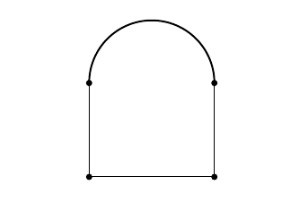
\includegraphics[scale = 1]{image5.PNG}
			\caption{Convex body with a face which is not exposed.}
		\end{center}
	\end{figure}
	
\end{remark}

\subsection{Polytopes and simple strongly isomorphic polytopes }

In this section, we define a subclass of convex bodies which are combinatorial in nature and allow us to approximate general convex bodies. We call a convex body $P \subseteq \RR^n$ a \textbf{polytope} if it can be written as the convex hull of a finite number of points. 

\begin{prop}[Properties of Polytopes]
	Let $P \subseteq \RR^n$ be an arbitrary polytope. Then, $P$ satisfies the following properties: 
	\begin{enumerate}[label = (\alph*)]
		\item The exposed faces of $P$ are exactly the faces of $P$. Moreover, $P$ has a finite number of faces. 
		\item Let $F_1, \ldots, F_k$ be the facets of $P$ with normal vectors $u_1, \ldots, u_k$. Then 
		\[
			P = \bigcap_{i = 1}^k H_{u_i, h_P(u_i)}^-
		\]
		In particular, the numbers $h_P(u_1), \ldots, h_P(u_k)$ determine $P$ uniquely. 

		\item The face poset $\mathcal{F}(P)$ of $P$ is a graded lattice which is graded by dimension. It satisfies the \textbf{Jordan-Dedekind chain condition}. In other words, if we have a face $F^j \in \mathcal{F}_j(P)$ and a face $F^k \in \mathcal{F}_k(P)$ satisfying $F^j \subset F^k$, then there are faces $F^i \in \mathcal{F}_i(P)$ for $j+1 \leq i \leq k-1$ such that 
		\[
			F^j \subset F^{j+1} \subset \ldots \subset F^{k-1} \subset F^k.
		\]
	\end{enumerate}
\end{prop}

\begin{proof}
	These properties follow from Corollary 2.4.2, Theorem 2.4.3, Corollary 2.4.4, and Corollary 2.4.8 in \cite{schneider_2013}. 
\end{proof}

We call a polytope $P \subseteq \RR^n$ \textbf{simple} if $\text{int} (P) \neq \emptyset$ and each of its vertices is contained in exactly $n$ facets. We say two polytopes $P_1, P_2$ are called \textbf{strongly isomorphic} if $\dim F_{P_1}(u) = \dim F_{P_2}(u)$ for all $u \in \RR^n \backslash \{0\}$. Strongly isomorphic polytopes have isomorphic face lattices where the isomorphism is given by matching faces which are cut out by support hyperplanes with the same normal vector. Moreover, the corresponding faces are also strongly isomorphic. 

\begin{lem}[Lemma 2.4.10 in \cite{schneider_2013}]
	If $P_1, P_2$ are strongly isomorphic polytopes, then for each $u \in \RR^n \backslash \{0\}$, the faces $F_{P_1}(u)$ and $F_{P_2}(u)$ are strongly isomorphic. 
\end{lem}
\begin{proof}
	See Lemma 2.4.10 in \cite{schneider_2013}. 
\end{proof}

We will be interested in approximating a set of convex bodies by polytopes which are simple and strongly isomorphic. To make sense of approximation of polytopes, we will equip the space of convex bodies with a metric.

\subsection{Hausdorff metric on convex bodies}

In this subsection, we equip the space of convex bodies $\mathsf{K}^n$ with the Hausdorff metric $\delta$. We define the \textbf{Hausdorff metric} of $K, L \in \mathsf{K}^n$ as 

Since convex sets are closed, it is Lebesgue measurable. Hence, it has a well-defined volume which we define as 
\begin{align*}
	\delta (K, L) & = \max \left \{ \sup_{x \in K} \inf_{y \in L} |x-y|, \sup_{y \in L} \inf_{x \in K} |x-y|\right \} \\
	& = \inf \{\varepsilon \geq 0 : K \subseteq L + \varepsilon B^n, L \subseteq K + \varepsilon B^n\} \\
	& = \norm{h_K - h_L}_\infty.
\end{align*}
For a proof of the equivalence of these three descriptions, we direct the reader to Theorem 3.2 in \cite{Hug2020-ue}. In Proposition~\ref{convex-body-is-metric-space}, we prove that $\delta$ is a metric on the space of convex bodies. In Theorem~\ref{approximation-SSI}, we prove that any set of convex bodies can be approximated by simple polytopes such that each simple polytope in the approximation are strongly isomorphic. 

\begin{prop} \label{convex-body-is-metric-space}
	The ordered pair $(\mathsf{K}^n, \delta)$ is a metric space. 
\end{prop}

\begin{proof}
	For $K, L, M \in \mathsf{K}^n$, we have 
	\[
		\delta(K, M) = \norm{h_K - h_M}_\infty \leq \norm{h_K - h_L}_\infty + \norm{h_L - h_M}_\infty = \delta(K, L) + \delta(L, M). 
	\]
	It is clear that $\delta (K, L) = \delta (L, K)$. Finally, we have $\delta(K, L) = 0$ if and only if $\norm{h_K - h_L}_\infty = 0$. Since $h_K$ and $h_L$ are continuous function, this is true if and only if $h_K = h_L$. Since $K$ and $L$ are the intersections of their support hyperplanes, this implies that $K = L$. This suffices for the proof. 
\end{proof}

\begin{thm}[Theorem 2.4.15 in \cite{schneider_2013}] \label{approximation-SSI}
	Let $K_1, \ldots, K_m \in \mathsf{K}^n$ be convex bodies. To every $\varepsilon > 0$, there are simple strongly isomorphic polytopes $P_1, \ldots, P_m$ such that $\delta (K_i, P_i) < \varepsilon$ for $i = 1, \ldots, m$.
\end{thm}

\begin{proof}
	See Theorem 2.4.15 in \cite{schneider_2013}. 
\end{proof}

In order for approximations to be useful, we need functions on $(\mathsf{K}^n, \delta)$ which are continuous. Since convex bodies are compact, they are also Lebesgue and Borel measurable. Thus, there is a well-defined function $\Vol_n : \mathsf{K}^n \to \RR_{\geq 0}$ defined by
\[
	\Vol_n (K) := \int_{x \in \RR^n} \1_K(x) \, d \lambda(x)
\]
where $\lambda$ is the Lebesgue measure on $\RR^n$. Then $\Vol_n(\cdot)$ is a continuous function on $(\mathsf{K}^n, \delta)$. For a proof of this fact, see Theorem 1.8.20 in \cite{schneider_2013}. For another example of a continuous map, consider the projection map $p : \mathsf{K}^n \times \RR^n \to \RR^n$ which maps $(K, x) \mapsto p(K, x)$ where $p(K, x)$ is the projection of $x$ onto $K$. For the proof that this map is continuous, see Section 1.8 in \cite{schneider_2013}. Finally, the map induced by the Minkowski sum $\mathsf{K}^n \times \mathsf{K}^n \to \mathsf{K}^n$ is continuous. 


\subsection{Mixed Volumes}

Recall that in the setting of mixed discriminants, for $n \times n$ matrices $A_1, \ldots, A_m$ we had the identity
\begin{equation} \label{ye-old}
	\det (\lambda_1 A_1 + \ldots + \lambda_m A_m) = \sum_{i_1, \ldots, i_n = 1}^m \lambda_{i_1} \ldots \lambda_{i_n} \cdot \mathsf{D}(A_{i_1}, \ldots, A_{i_n})
\end{equation}
where the multilinear form $\mathsf{D}$ was the mixed discriminant. In this subsection, we aim to achieve a similar expression in the world of convex bodies. That is, for convex bodies $K_1, \ldots, K_m \subseteq \RR^n$, we want to expand $\Vol_n(\lambda_1 K_1 + \ldots + \lambda_m K_m)$ as a homogeneous polynomial. 
\begin{example}
	Let $K \subseteq \RR^2$ be a polygon and $L \subseteq \RR^2$ be the unit disc. Then by drawing $\lambda K + \mu L$ on the plane, we can compute 
	\[
		\Vol_2 (\lambda K + \mu L) = \lambda^2 \Vol_2(K) + \lambda \mu \cdot \mathsf{perimeter}(K) + \mu^2 \Vol_2(L). 
	\]
	This provides some evidence of a expansion of the form Equation~\ref{ye-old} since the coefficients seem to encode geometric information about the convex bodies $K$ and $L$. 
\end{example}

\begin{defn}
	For $n \geq 2$, let $P_1, \ldots, P_n \subseteq \RR^n$ be polytopes and let $\mathcal{U}$ be the set of unit facet normals of $P_1 + \ldots + P_{n-1}$. We define their mixed volume $\mathsf{V}_n(P_1, \ldots, P_n)$ inductively by 
	\[
		\mathsf{V}_n(P_1, \ldots, P_n) = \frac{1}{n} \sum_{u \in \mathcal{U}} h_{P_n}(u) \cdot \mathsf{V}_{n-1} (F_{P_1}(u), \ldots, F_{P_{n-1}}(u)).
	\]
	On the right hand side of the equation though $F_{P_1}(u), \ldots, F_{P_{n-1}}(u)$ are in $\RR^n$, since they are in parallel hyperplanes we can consider them as subsets of $\RR^{n-1}$ by projecting them orthogonally on the same hyperplane isomorphic to $\RR^{n-1}$. Thus, the mixed volume $\mathsf{V}_{n-1}(F_{P_1}(u), \ldots, F_{P_{n-1}}(u))$ is well-defined. For $n = 1$, we define $V_1 ([a, b]) = b-a$. 
\end{defn}

\begin{thm}[Theorem 3.7 in \cite{Hug2020-ue}]
	For polytopes $P_1, \ldots, P_m \subseteq \RR^n$ be polytopes. Then, we have 
	\[
		\Vol_n(\lambda_1 P_1 + \ldots + \lambda_m P_m) = \sum_{i_1, \ldots, i_n = 1}^m \lambda_{i_1} \ldots \lambda_{i_n} \cdot \mathsf{V}_n (P_{i_1}, \ldots, P_{i_n}).
	\]
\end{thm}

From this formula, it is not difficult to prove the following inversion formula:
\[
	\mathsf{V}_n(P_1, \ldots, P_n) = \frac{1}{n!} \sum_{k = 1}^n (-1)^{n+k} \sum_{1 \leq r_1 < \ldots < r_k \leq n} \Vol_n (P_{r_1} + \ldots + P_{r_k}).
\]
For a proof of this formula, see Theorem 3.8 in \cite{Hug2020-ue}. This formula implies that we can continuously extend $\mathsf{V}_n$ to arguments in $\mathsf{K}^n$ since $\Vol_n$ and Minkowski sum are continuous on the space of convex bodies. We call the resulting value $\mathsf{V}_n (K_1, \ldots, K_n)$ the \textbf{mixed volume} of $K_1, \ldots, K_n$. From continuity, we have the following theorem. 
\begin{thm}
	Let $K_1, \ldots, K_m \subseteq \RR^n$ be convex bodies. Then, we have 
	\[
		\Vol_n (\lambda_1 K_1 + \ldots + \lambda_m K_m) = \sum_{i_1 , \ldots , i_n = 1}^m \lambda_{i_1} \ldots \lambda_{i_n} \cdot \mathsf{V}_n (K_{i_1}, \ldots, K_{i_n}).
	\]
\end{thm}

\chapter{Mechanisms for Log-concavity}

\section{Log-Concavity and Ultra Log-Concavity}

\begin{defn}

\end{defn}

(Many sequences in combinatorics are proven to be log-concave ... give examples: Read's conjecture, Mason's Conjecture, etc. )
\section{Alexandrov's Inequality for Mixed Discriminants}

In this section we introduce a fundamental inequality given in Theorem~\ref{A-Inequality-MIXED-DISCRIMINANT} in the theory of mixed discriminants. This inequality is similar to the inequality for mixed volumes of convex bodies given in Theorem~\ref{AF-inequality}. We first give a generalization of this inequality to the larger class of objects called \textbf{hyperbolic polynomials}. For an introduction to the theory of hyperbolic polynomials, we refer the reader to \cite{schneider_2013} and \cite{hyperbolic-polynomials}. We call a homogeneous polynomial $p \in \RR[x_1, \ldots, x_n]$ \textbf{hyperbolic in direction} $v$ for $v \in \RR^n$ if and only if $p(v) > 0$ and for each $x \in \RR^n$, the univariate polynomial $p(x + tv)$ when considered a polynomial in $t$ has only real roots. If $p$ is hyperbolic in direction $v \in \RR^n$ then we can define the hyperbolicity cone $\mathcal{H} (p)$ as the set of directions for which $p$ is hyperbolic. 

\begin{thm}[Theorem 5.5.3 in \cite{schneider_2013}]
	Let $p$ be a hyperbolic homogeneous polynomial of degree $k \geq 1$ on $\RR^n$, and let $\tilde{p}$ be its polarization. Let $y, x_2, \ldots, x_k \in \mathcal{H}(p)$, $x \in \overline{\mathcal{H}(p)}$, and $z \in \RR^n$. Then 
	\[
		\widetilde{p}(y, z, x_3, \ldots, x_k)^2 \geq \widetilde{p}(y, y, x_3, \ldots, x_k) \widetilde{p} (z, z, x_3, \ldots, x_k).
	\]
\end{thm}

\begin{proof}
	See Theorem 5.5.3 in \cite{schneider_2013}.
\end{proof}

\begin{thm} [Alexandrov's Inequality for Mixed Discriminants] \label{A-Inequality-MIXED-DISCRIMINANT}
	Let $X, Y, A_1, \ldots, A_{n-2}$ be real symmetric positive definite $n \times n$ matrices. Then 
	\[
		\mathsf{D}(X, Y, A_1, \ldots, A_{n-2})^2 \geq \mathsf{D}(X, X, A_1, \ldots, A_{n-2}) \cdot \mathsf{D} (Y, Y, A_1, \ldots, A_{n-2})
	\]
	where equality holds if and only if $B = \lambda A$ for a real number $\lambda$. 
\end{thm}

\begin{cor} \label{mixed-discriminant-log-concave-sequence}
	Let $A, B$ be $n \times n$ positive definite symmetric real matrices. For $0 \leq k \leq n$, define the mixed discriminant
	\[
		D_k := \mathsf{D} (\underbrace{A, \ldots, A}_{k \text{ times}}, \underbrace{B \ldots, B}_{n-k \text{ times}}).
	\]
	Then the sequence $D_0, D_1, \ldots, D_n$ is log-concave. 
\end{cor}

\begin{cor}
	Let $A, B, D_k$ for $1 \leq k \leq n$ be as in Corollary~\ref{mixed-discriminant-log-concave-sequence}. If $D_k^2 = D_{k-1}D_{k+1}$ for some $1 \leq k \leq n-1$, then $D_k^2 = D_{k-1} D_{k+1}$ holds for all $k = 1, \ldots, n-1$. 
\end{cor}

\begin{proof}
	This follows from the equality case in Theorem~\ref{A-Inequality-MIXED-DISCRIMINANT}. 
\end{proof}
\section{Alexandrov-Fenchel Inequality}

\begin{thm}[Alexandrov-Fenchel Inequality] \label{AF-inequality}
	Let $K_1, K_2, \ldots, K_{d-2} \subseteq \RR^d$ be convex bodies. For any convex bodies $X, Y \subseteq \RR^d$, we have the inequality
	\[
		\mathsf{V}_d(X, Y, K_1, \ldots, K_{d-2})^2 \geq \mathsf{V}_d(X, X, K_1, \ldots, K_{d-2}) \cdot \mathsf{V}_d(Y, Y, K_1, \ldots, K_{d-2}). 
	\]
\end{thm}

\begin{proof}
	
\end{proof}

\section{Lorentzian Polynomials}

Our main reference for Lorentzian polynomials is \cite{lorentzian-polynomials}. Following the notation in \cite{lorentzian-polynomials}, we let $H_n^d$ be the space of degree $d$ homogeneous polynomials in $n$ variables with real coefficients equipped with the Euclidean topology with respect to the coefficients.  
\begin{defn}
	Let $\underbar{L}_n^2 \subseteq H_n^2$ be the open subset of quadratic forms with positive coefficients and Hessian with signature $(+, -, \ldots, -)$. For $d \geq 3$, we define 
	\[
		\underbar{L}_n^d := \{f \in H_n^d : \partial_i f \in \underbar{L}_n^{d-1} \text{ for all $i$}\}.
	\] 
	We call polynomials in $\underbar{L}_n^d$ \textbf{strictly Lorentzian}.
\end{defn}

\begin{defn}
	A polynomial $f \in \RR[w_1, \ldots, w_n]$ is \textbf{stable} if $f$ is non-vanishing on $\mathbb{H}^n$ where $\mathbb{H}$ is the open upper half plane in $\mathbb{C}$. Following \cite{milnor-numbers}, we denote by $S_n^d$ the set of degree $d$ homogeneous stable polynomials in $n$ variables 
\end{defn}

\begin{defn}
	We define $J \subseteq \NN^n$ to be \textbf{$M$-convex} if for any $\alpha, \beta \in J$ and any index $i$ satisfying $\alpha_i > \beta_i$, there is an index $j$ satisfying $\alpha_j < \beta_j$ and $\alpha - e_i + e_j \in J$. 
\end{defn}

\begin{defn}
	For any polynomial $f \in \RR[x_1, \ldots, x_n]$ we define $\text{supp}(f) := \{\alpha \in \NN^n : c_\alpha \neq 0\}$ where $c_\alpha$ is the coefficient in front of $x^\alpha$ in $f$. 
\end{defn}

\begin{defn}
	Let $M_n^d$ be the set of degree $d$ homogeneous polynomials in $\RR_{\geq 0}[x_1, \ldots, x_n]$ whose supports are $M$-convex.  
\end{defn}



\begin{defn}[Definition 2.6 in \cite{lorentzian-polynomials}]
	We set $L_n^0 = S_n^0$, $L_n^1 = S_n^1$, and $L_n^2 = S_n^2$. For $d \geq 3$, we define 
	\[
		L_n^d = \{f \in M_n^d : \partial_i f \in L_n^{d-1} \text{ for all } i \in [n]\}.
	\]
	The set $L_n^d$ consists of homogeneous degree $d$ polynomials with non-negative coefficients whose supports are $M$-convex such that for all $\alpha \in \Delta_n^{d-2}$, we have that $\partial^\alpha f$ is a stable quadratic form. 
\end{defn}

\begin{defn} \label{defn-lorentzian}
	We call a homogeneous polynomial $f \in \RR_{\geq 0}[x_1, \ldots, x_n]$ of degree $d$ Lorentzian if it satisfies any of the following equivalent conditions:
	\begin{enumerate}[label = (\roman*)]
		\item The polynomial $f$ is the closure of $\underbar{L}_n^d \subseteq H_n^d$. 

		\item The polynomial $f \in L_n^d$. 

		\item For any $\alpha \in \NN^n$ with $|\alpha| \leq d-2$, the polynomial $\partial^\alpha f$ is identically zero or log-concave at any $a \in \RR_{>0}^n$. 
	\end{enumerate}
\end{defn}

In the literature, condition (iii) in Definition~\ref{defn-lorentzian} is also known as \textbf{strong log-concavity} \cite{strongly-log-concave}. These conditions are proven to be equivalent in \cite{lorentzian-polynomials}. 

\begin{prop}[Proposition 4.5 in \cite{lorentzian-polynomials}]
	If $f$ is Lorentzian, then for any $v_1 \in \RR^n$ and $v_2, \ldots, v_d \in \RR_{\geq 0}^n$, we have that 
	\[
		\widetilde{f}(v_1, v_2, v_3, \ldots, v_d)^2 \geq \widetilde{f}(v_1, v_1, v_3, \ldots, v_d) \cdot \widetilde{f}(v_2, v_2, v_3, \ldots, v_d)
	\]
	where $\widetilde{f}$ denotes the polarization of $f$. 
\end{prop}

\section{Combinatorial Atlas}

\chapter{Log-concavity Results for Posets and Matroids}

\section{Stanley's Poset Inequality}

\section{Stanley's Matroid Inequality} 

\section{Kahn-Saks Inequality}


\chapter{Hard Lefschetz Property and Hodge-Riemann Relations}

\section{Gorenstein ring associated to a polynomial}

In this section, we study a ring introduced in by Toshiaki Maeno and Yasuhide Numata in \cite{MN-gorenstein}. The Gorenstein Ring associated to the basis generating polynomial of a matroid is intimately related to graded Mobius(") algebra associated to a matroid and the Chow ring associated to a matroid. The Gorenstein stein ring associated to a polynomial is defined based on the action of differential forms on a fixed homogeneous polynomial.

\begin{defn}
	Let $f \in \RR[x_1, \ldots, x_n]$ be a homomgeneous polynoimal and let $S := \RR[\partial_1, \ldots, \partial_n]$ be the polynomial ring of differentials where $\partial_i := \partial_{x_i}$. We define the ring 
	\[
		A_f^\bullet := S / \Ann_S (f).
	\]
	We call $A_f^\bullet$ the Gorenstein ring associated to the polynomial $f$. Alternatively, we view the polynomial ring $\RR[x_1, \ldots, x_n]$ as a module over the polynomial ring $\RR[X_1, \ldots, X_n]$ where the module structure is defined by the relation
	\[
		p(X_1, \ldots, X_n) \cdot q(x_1, \ldots, x_n) := p(\partial_1, \ldots, \partial_n) q(x_1, \ldots, x_n). 
	\]
	Then the Gorenstein ring can be equivalently defined as $\RR[X_1, \ldots, X_n] / \Ann (f)$. Note that this is trivially equivalent to the first definition. We note this alternative perspective because both conventions are used in the literature \cite{MNY,MN-gorenstein}. 
\end{defn}

The Gorenstein ring associated to a polynomial has a natural grading with respect to the degree of the differential form. Before we prove that this actually gives $A_f^\bullet$ a graded ring structure, we first prove Lemma~\ref{homogeneous-parts}.

\begin{lem} \label{homogeneous-parts}
	Let $\xi \in \RR[\partial_1, \ldots, \partial_n]$ and $f \in \RR[x_1, \ldots, x_n]$ be a homogeneous polynomial. We can decompose $\xi = \xi_0 + \xi_1 + \ldots$ into its homogeneous parts. If $\xi (f) = 0$, then $\xi_d (f) = 0$ for all $d \geq 0$. 
\end{lem}

\begin{proof}
	Let $d = \deg (f)$. If $\xi_i (f) \neq 0$, then $i \leq d$ and $\xi_i(f)$ is a homomgeneous polynomial of degree $d-i$. Thus, 
	\[
		\xi (f) = \xi_0 (f) + \xi_1(f) + \ldots
	\]
	will be the homomgeneous decomposition of the polynomial $\xi(f)$. Since this is equal to $0$, all components of the decomposition are equal to zero. This proves the proposition. 
\end{proof}

\begin{prop}
	The Chow ring $A_f^\bullet$ is a graded $\RR$-algebra where $A_f^k$ consists of the forms of degree $k$. 
\end{prop}

\begin{proof}
	Let us define $A_f^k$ as in the statement of the lemma. Let $d = \deg (f)$ be the degree of the homomgeneous polynomial. Whenver $k > d$, the ring $A_f^k$ is clearly trivial. From Lemma~\ref{homogeneous-parts}, we have the direct sum decomposition 
	\[
		A_f^\bullet = \bigoplus_{k = 0}^d A_f^k.
	\]
	It is also clear that multiplication induces maps $A_f^r \times A_f^s \to A_f^{r+s}$ for all $r, s \geq 0$.
\end{proof}

The following result (Proposition (CITE)) is well-known and it follows from Theorem 2.1 in CITE(Maeno, Watanabe, Lefschetz elements of ARtinian Gorenstein algebras and Hessians of homogeneous polynomials)
\begin{prop} \label{chow-ring-is-a-PD-algebra}
	Let $f$ be a homogeneous polynoimal of degree $d$. Then, the ring $A_f^\bullet$ is a Poincare-Duality algebra. That is, the ring satisfies the following two properties:
	\begin{enumerate}[label = (\alph*)]
		\item $A_f^d \simeq A_f^0 \simeq \RR$;

		\item The pairing induced by multiplication $A_f^{d-k} \times A_f^k \to A_f^d \simeq \RR$ is non-degenerate for all $0 \leq k \leq d$. 
	\end{enumerate}
\end{prop}

We first make a small remark on non-degeneracy to make it clear what we mean when we say a pairing is non-degenerate. 
\begin{lem} \label{non-degeneracy-definition}
	Let $B : V \times W \to k$ be a bilinear pairing between two finite-dimensional $k$-vector spaces $V$ and $W$. Then, any two of the following three conditions imply the third. 
		\begin{enumerate}[label = (\roman*)]
			\item The map $B_V : V \to W^*$ defined by $v \mapsto B(v, \cdot)$ has trivial kernel.
			\item The map $B_W : W \to V^*$ defined by $w \mapsto B(\cdot, w)$ has trivial kernel. 
			\item $\dim V = \dim W$. 
		\end{enumerate}
	\end{lem}

	\begin{proof}
		Condition (i) implies $\dim V \leq \dim W$ and Condition (ii) implies $\dim W \leq \dim V$. Thus (i) and (ii) both imply (iii). Now, suppose that (i) and (iii) are true. Then $B_V$ is an isomorphism between $V$ and $W*$ [3.69 in Axler (CITE???)]. Let $v_1, \ldots, v_n$ be a basis for $V$. Then $B_V(v_1), \ldots, B_V(v_n)$ is a basis of $W^*$. Let $w_1, \ldots, w_n$ be the dual basis in $W$ with respect to this basis of $W^*$. Suppose that $\sum \lambda_i w_i \in \ker B_W$. Then for all $v \in V$, we have 
		\[
			\sum_{i = 1}^n \lambda_i B_V(v)(w) = B \left ( v, \sum_{i = 1}^n \lambda_i w_i \right ) = 0. 
		\]
		By letting $v = v_1, \ldots, v_n$, we get $\lambda_i = 0$ for all $i$. 
	\end{proof}

We say a pairing between finite-dimensional vector spaces is non-degenerate whenever all three conditions in Lemma~\ref{non-degeneracy-definition} hold. As a corollary, we have the following result.

\begin{cor} \label{same-dimensions}
	Let $f$ be a homogeneous polynomial of degree $d \geq 2$ and let $k$, $0 \leq k \leq d$, by a non-negative integer. Then $\dim_\RR A_f^k = \dim_\RR A_f^{d-k}$. 
\end{cor}

In Proposition(CITE), we can define $\deg_f : A_f^d \to \RR$ to be the isomorphism defined by evaluation at $f$. That is, for any $\xi \in A_f^d$, we can define $\deg_f (\xi) := \xi(f)$ where $\xi$ acts on $f$ by differentiation. FOllowing (CITE HODGE THEORY OF COMBINATORIAL GEOMETRIES), we formulate the following definition

\begin{defn}
	Let $f$ be a homogeneous polynomial of degree $d$ and let $k \leq d/2$ be a non-negative integer. For an element $l \in A_f^1$, we define the following notions:
	\begin{enumerate}[label = (\alph*)]
		\item The \textbf{Lefschetz operator} on $A_f^k$ associated to $l$ is the map $L_l^k : A_f^k \to A_f^{d-k}$ defined by $\xi \mapsto l^{d-2k} \cdot \xi$. 

		\item The \textbf{Hodge-Riemann form} on $A_f^k$ associated to $l$ is the bilinear form $Q_l^k : A_f^k \times A_f^k \to \RR$ defined by $Q_l^k (\xi_1, \xi_2) = (-1)^k \deg (\xi_1 \xi_2 l^{d-2k})$.

		\item The \textbf{primitive subspace} of $A_f^k$ associated to $l$ is the subspace
		\[
			P_l^k := \{\xi \in A_f^k : l^{d-2k+1} \cdot \xi = 0\} \subseteq A_f^k.
		\]
	\end{enumerate}
\end{defn}

\begin{defn}
	Let $f$ be a homogeneous polynomial of degree $d$, let $k \leq d/2$ be a non-negative integer, and let $l \in A_f^1$ be a linear differential form. We define the following notions:
	\begin{enumerate}[label = (\alph*)]
		\item (Hard Lefschetz Property) We say $A_f$ satisfies $\HL_k$ with respect to $l$ if the Lefschetz operator $L_l^k$ is an isomorphism.

		\item (Hodge-Riemann Relations) We say $A_f$ satisfies $\HRR_k$ with respect to $l$ if the Hodge-Riemann form $Q_l^k$ is positive definite on the primitive subspace $P_l^k$. 
	\end{enumerate}
\end{defn}

Sometimes, instead of saying $A_f$ satisfies Hodge-Riemann Relations or the Hard Lefschetz Property, we will say that $f$ satisfies Hodge-Riemann Relations or the Hard Lefschetz property. For any $a \in \RR^n$, we can define the linear differential form $l_a := a_1 \partial_1 + \ldots + a_n \partial_n$. We say that $f$ satisfies $\HL$ or $\HRR$ with respect to $a$ if and only if it satisfies $\HL$ or $\HRR$ with respect to $l_a$. Most applications of the Hodge-Riemann Relations only end up using the relations up to degree $k \leq 1$. (GIVE EXAMPLE OF AN APPLICATION WHICH USES HIGHER DIMENSION,, maybe Chris Eur???) 

\begin{prop} [Lemma 3.4 in \cite{MNY}] \label{conditions-for-HL-HRR}
	Let $f \in \RR[x_1, \ldots, x_n]$ be a homogeneous polynomial of degree $d \geq 2$ and $a \in \RR^n$. Assume that $f(a) > 0$. Then, 
	\begin{enumerate}[label = (\alph*)]
		\item $A_f$ has $\HL_1$ with respect to $l_a$ if and only $Q_{l_a}^1$ is non-degenerate. 

		\item Suppose that $A_f$ satisfies $\HL_1$. Then $A_f$ has $\HRR_1$ with respect to $l_a$ if and only if $-Q_{l_a}^1$ has signature $(+, -, \ldots, -)$. 
	\end{enumerate}
\end{prop}

\begin{proof}
	We include a proof for completeness. We first prove the statement in (a). Suppose that $A_f$ has $\HL_1$ with respect to $l_a$. We have the following commutative diagram:
	\[\begin{tikzcd}
	{A_f^1 \times A_f^1} && {A_f^1 \times A_f^{d-1}} \\
	& {\mathbb{R}}
	\arrow["{\text{id} \times L_{l_a}^1}", from=1-1, to=1-3]
	\arrow["{-Q_{l_a}^1}"', from=1-1, to=2-2]
	\arrow[from=1-3, to=2-2]
\end{tikzcd}\]
where the missing mapping is multiplication. If $A_f$ has $\HL_1$ with respect to $l_a$, then the top map between $A_f^1 \times A_f^1 \to A_f^1 \times A_f^{d-1}$ is an bijection. Thus the non-degeneracy of $Q_{l_a}^1$ follows from the non-degeneracy of the multiplication pairing as stated in Proposition~\ref{chow-ring-is-a-PD-algebra}. Now, suppose that $Q_{l_a}^1$ is non-degenerate. Then, the map $B : A_f^1 \to (A_f^1)^*$ defined by $\xi \mapsto -Q_{l_a}^1(\xi, \cdot)$ is given by $m(L_{l_a}^1 \xi, \cdot)$ where $m : A_f^1 \to A_f^{d-1} \to \RR$ is the multiplication map. This is the composition of $A_f^1 \to A_f^{d-1} \to (A_f^1)_*$ where the first map is $L_{l_a}^1$ and the second map is injective from the non-degeneracy of the multiplication map. This proves that $L_{l_a}^1$ is injective. From Corollary~\ref{same-dimensions}, the map $L_{l_a}^1$ is an isomorphism. This suffices for the proof of (a). \\

To prove (b), consider the commutative diagram
\[\begin{tikzcd}
	{\mathbb{R}} & {A^0_f} & {A_f^1} & {A_f^{d-1}} & {A_f^d} & {\mathbb{R}}
	\arrow["{\times l_a}", from=1-2, to=1-3]
	\arrow["{L_{l_a}^1}", from=1-3, to=1-4]
	\arrow["{\times l_a}", from=1-4, to=1-5]
	\arrow["\simeq", from=1-1, to=1-2]
	\arrow["\simeq", from=1-5, to=1-6]
	\arrow["L_{l_a}^0"{description}, bend right= 18, from=1-2, to=1-5]
\end{tikzcd}\]
Note that $L_{l_a}^0$ is an isomorphism because 
\[
	\deg L_{l_a}^0 (1) = l_a^d (f)  = d! f(a) \neq 0.
\]
Thus, we have $A_f^1 = \RR l_a \oplus P_l^1$ where the direct sum is orthogonal over the Hodge-Riemann form by definition of the primitive subspace. Now, note that 
\[
	-Q_{l_a}^1(l_a, l_a) = l_a^d (f) = -d! f(a) > 0. 
\]
Thus, the signature of $-Q_{l_a}^1$ is $(+, -, \ldots, -)$ if and only if $Q_{l_a}^1$ is positive definite over the primitive subspace if and only if $A_f$ satisfies $\HRR_1$ with respect to $l_a$. 
\end{proof}

From Sylvester's Law of Inertia and the fact that is Hessians of Lorentzian polynomials always have at most one positive eigenvalue on the positive orthant. (cite in previous part of thesis maybe)
\begin{lem}[Lemma 3.5 in \cite{MNY}] \label{lorentzian-HL-iff-HRR}
	If $f \in \RR [x_1, \ldots, x_n]$ is Lorentzian, then for any $a \in \RR_{\geq 0}^n$ with $f(a) > 0$, $A_f^1$ has $\HL_1$ with respect to $l_a$ if and only if $f$ has the $\HRR_1$ with respect to $l_a$. 
\end{lem}
\section{Local Hodge-Riemann Relations}

Suppose that we are trying to prove the Hodge-Riemann Relations property for a Lorentzian polynomial. To do so, it is actually enough to show that it satisfies a ``local'' version of the Hodge-Riemann relations. This will imply that it satisfies the Hard Lefschetz Property, which by Lemma~\ref{lorentzian-HL-iff-HRR} is enough to prove that it satisfies Hodge-Riemann relations. We define the local $\HRR$ as in \cite{MNY}. 

\begin{defn}
	A homogeneous polynomial $f \in \RR[x_1, \ldots, x_n]$ of degree $d \geq 2k+1$ satisfies the \textbf{local} $\HRR_k$ with respect to a form $l \in A_f^1$ if for all $i \in [n]$, either $\partial_i f = 0$ or $\partial_i f$ satisfies $\HRR_k$ with respect to $l$. 
\end{defn}

One existing inductive mechanism for proving Hodge-Riemann relations is Lemma~\ref{local-hrr-mechanism}. 

\begin{lem} [Lemma 3.7 in \cite{MNY}] \label{local-hrr-mechanism}
	Let $f \in \RR_{\geq 0}[x_1, \ldots, x_n]$ be a homogeneous polynomial of degree $d$ and $k$ a positive integer with $d \geq 2k+1$, and $a = (a_1, \ldots, a_n) \in \RR^n$. Suppose that $f$ has the local $\HRR_k$ with respect to $l_a$. 
	\begin{enumerate}[label = (\roman*)]
		\item If $a \in \RR_{> 0}^n$, then $A_f$ has the $\HL_k$ with respect to $l_a$. 
		\item If $a_1 = 0, a_2, \ldots, a_n > 0$ and $\{\xi \in A_f^k : \partial_i \xi = 0 \text{ for $i = 2, \ldots, n$}\} = \{0\}$, then $A_f$ has the $\HL_k$ with respect to $l_a$. 
	\end{enumerate}
\end{lem}

This is effective in proving that all Lorentzian polynomials satisfy $\HRR_1$ with respect to $l_a$ for any $a \in \RR^n_{> 0}$. Indeed, this is easy to prove for Lorentzian polynomials of small degree. For an arbitrary Lorentzian polynomial, all of its partial derivatives are also Lorentzian (CITE THIS RESULT SOMEWHERE IN THE THESIS). Thus, by the inductive hypothesis all of these polynomials satsisfy $\HRR_1$. But this implies from Lemma~\ref{local-hrr-mechanism} that the original polynomial satisfies $\HL_1$, hence $\HRR_1$ since it is Lorentzian. This proves Theorem~\ref{lorentzian-satisfies-HRR}.

\begin{thm} [Theorem 3.8 in \cite{MNY}] \label{lorentzian-satisfies-HRR}
	If $f \in \RR[x_1, \ldots, x_n]$ is Lorentzian, then $f$ has $\HRR_1$ with respect to $l_a$ for any $a \in \RR_{> 0}^n$. 
\end{thm}

If the value of $a$ is not restricted to the positive orthant and additionally we know that $\partial_1, \ldots, \partial_n$, then we have the following computational result. 

\begin{cor} \label{partial-independent-implies-hessian}
	Let $f$ be a homogeneous polynomial of degree $d \geq 2$. If $\partial_1 f, \ldots, \partial_n f$ are linearly independent in $\RR[x_1, \ldots, x_n]$ and $f(a) > 0$ for some $a \in \RR^n$, then $A_f$ satisfies $\HRR_1$ with respect to $l_a$ if and only if $\Hess_f|_{x = a}$ has signature $(+, -, \ldots, -)$. 
\end{cor}

\begin{proof}
	Since $\partial_1 f_1, \ldots, \partial_n f_n$ are linearly independent, the partials $\partial_i$ form a basis for $A_f^1$. Thus, the signature of $Q_{l_a}^1$ is actually the signature of matrix of $Q_{l_a}^1$ with respect to the set $\{\partial_1, \ldots, \partial_n\}.$ We have 
	\[
		-Q_{l_a}^1(\partial_i, \partial_j) = \partial_i \partial_j l_a^{d-2} f =  l_a^{d-2} \partial_i \partial_j f = (d-2)! \partial_i \partial_j f(a).
	\]
	This proves that the signature of $-Q^1_{l_a}$ is the same as the signature of $\Hess_f |_{x = a}$.  We are done from Lemma~\ref{conditions-for-HL-HRR}(b).
\end{proof}
\section{The Gorenstein ring associated to the basis generating polynomial of a matroid}

\begin{defn}
	Let $M$ be a matroid. We define $A^\bullet(M) := A^\bullet_{f_M}$ to be the \textbf{Gorenstein ring associated to the basis generating polynomial} of $M$. In this case, we define 
	\[
		S_M := \RR [ \partial_e : e \in E]
	\]
	to be the polynomial ring in variables indexed by the ground set. We also define
	\[
		\Ann_M := \Ann_{S_M}(f_M)
	\]
	which is the annihilator of $f_M$ with respect to $S_M$. Then $A(M) = S_M / \Ann_M$. 
\end{defn}

\begin{remark}
	For the sake of brevity, we will refer to the ring $A(M)$ as simply the \textbf{Gorenstein ring} of the matroid $M$. As a warning, note that this is not standard in the literature since there are \textbf{many} Gorenstein rings associated to matroids. Immediate examples are the Chow ring and augmented Chow ring of a matroid \cite{huh-semi-small}. 
\end{remark}

We will now prove that the Gorenstein ring associated to the basis generating polynomial of matroid only depends on its simplification. Indeed, if $a, b \in E(M)$ are parallel elements, then $\partial_a - \partial_b$ gets annihilated and if $e \in E(M)$ is a loop then $\partial_e$ gets annihilated. We will describe this isomorphism in Theorem~\ref{only-simplification-matters}. Before proving this result, we first describe some common elements in the ideal $\Ann_M$. 

\begin{prop}[Proposition 3.1 in \cite{MN-gorenstein}]
	The annihilator $\Ann_M$ contains the elements
	\[
		\Lambda_M := \{x_e^2 : e \in E(M)\} \cup \{x^S : S \notin \mcI (M)\} \cup \{x^A - x^{A'} : A, A' \in \mcI(M), \overline{A} = \overline{A'}\}.
	\]
\end{prop}



\begin{example}
	The elements $\Lambda_M$ unfortunately do not generate $\Ann_M$ in general. In \cite{MN-gorenstein}, they give an example of matroid which is the matroid described by the linear independence of the following five vectors. 
	\begin{align*}
	 	e_1 & = (1, 0, 0) \\
	 	e_2 & = (0, 1, 0) \\
	 	e_3 & = (0, 0, 1) \\
	 	e_4 & = (1, 1, 0) \\
	 	e_5 & = (0, 1, 1).
	\end{align*}
	The bases are $123, 125, 134, 135$, and $145$. From Example 3.5 in \cite{MN-gorenstein}, it happens that 
	\[
		\Ann_M = \langle \Lambda_M \rangle + (\partial_1 \partial_3 + \partial_{4} \partial_5 - \partial_1 \partial_5 - \partial_3 \partial_4).
	\]
\end{example}


Let $M = (E, \mathcal{I})$ be a matroid and let $\widetilde{M}$ be its simplification. Recall that $\widetilde{M}$ is a matroid on the ground set of rank-$1$ flats $E(\widetilde{M}) = \{\bar{x} : x \in E(M) \backslash E_0 (M)\}$ whose independent sets consist of the subsets of $E(\widetilde{M})$ where by taking one representative from each rank-$1$ flat, we get an independent set of $M$. We can define $\phi : S_M \to S_{\widetilde{M}}$ and $\psi : S_{\widetilde{M}} \to S_M$ by 
\begin{align*}
	\phi (\partial_{x_e}) := \partial_{\overline{x_e}}, \quad \text{and} \quad \psi (\partial_{\overline{x}}) := \frac{1}{|\overline{x}|} \sum_{e \in \overline{x}} \partial_{x_e}.
\end{align*}
The entire maps $\phi$ and $\psi$ are then defined by using the universal property of polynomial rings to extend over the whole space. 

\begin{thm} \label{only-simplification-matters}
	The maps $\phi : S_M \to S_{\widetilde{M}}$ and $\psi : S_{\widetilde{M}} \to S_M$ induce isomorphisms between $A(M)$ and $A(\widetilde{M})$. 
\end{thm}

\begin{proof}
	We first prove that $\phi$ and $\psi$ induce homomorphisms between the Chow rings. To show that $\phi$ induces a homomorphism, consider the diagram in Equation~\ref{extension-1}.
	\begin{equation} \label{extension-1}
			\begin{tikzcd}
				{S_M} && {S_{\widetilde{M}}} && {A(\widetilde{M})} \\
				\\
				&& {A(M)}
				\arrow["\phi", from=1-1, to=1-3]
				\arrow["{\pi_{\widetilde{M}}}", from=1-3, to=1-5]
				\arrow["{\pi_M}"', from=1-1, to=3-3]
				\arrow["{\exists ! \Phi}"', dotted, from=3-3, to=1-5]
			\end{tikzcd}
	\end{equation}
		

Let $\xi \in S_M$ be an element satisfying $\xi (f_M) = 0$. We will prove that $\phi(\xi) (f_{\widetilde{M}}) = 0$. In other words, we want to prove that $\Ann_M \subseteq \ker \pi_{\widetilde{M}} \circ \phi$. From Proposition~\ref{homogeneous-parts}, it suffices to consider the case where $\xi$ is homogeneous. Let $e_1, \ldots, e_s$ be representatives of all parallel classes. Then, we have that $M = \overline{e_1} \sqcup \ldots \sqcup \overline{e_s} \cup E_0$ where $E_0$ denotes the loops in $M$. In terms of the basis generating polynomials, we have 
\begin{align*}
	f_{\widetilde{M}}(x_{\overline{e_1}}, \ldots, x_{\overline{e_s}}) & = \sum_{\substack{1 \leq i_1 < \ldots < i_r \leq s \\ \{\overline{e_{i_1}}, \ldots, \overline{e_{i_r}}\} \in \mathcal{B}(\widetilde{M})}} x_{\overline{e_{i_1}}} \ldots x_{\overline{e_{i_r}}} \\ 
	f_M(x_1, \ldots, x_n) & = f_{\widetilde{M}} \left ( y_1, \ldots, y_s \right )
\end{align*}
where for $1 \leq i \leq s$, we define $y_i := \sum_{e \in \overline{e_i}} x_e$. Since $\xi$ is homogeneous of degree $k$, we can write it in the form $\xi = \sum_{\substack{\alpha \subseteq [n] \\ |\alpha| = k}} c_\alpha \partial^\alpha$. Then, we have 
\begin{align} \label{karen}
	\xi (f_M) & = \sum_{\beta \in \mathcal{B}} \xi (x^\beta) = \sum_{\beta \in \mathcal{B}(M)} \sum_{\substack{\alpha \subseteq [n] \\ |\alpha| = k}} c_\alpha \partial^\alpha x^\beta = \sum_{\gamma \in \mathcal{I}_{r-k}(M)} \left ( \sum_{ \substack{\alpha \in \mathcal{I}_k \\ \alpha \cup \gamma \in \mathcal{I}_r(M)}} c_\alpha  \right ) x^\gamma. 
\end{align}

Since $\xi(f_M) = 0$, we know that all of the coefficients on the right hand side of Equation~\ref{karen} are equal to $0$. Thus, for any $\gamma \in \mathcal{I}_{r-k}(M)$, we have 
\[
	\sum_{\substack{\alpha \in I_k \\ \alpha \cup \gamma \in \mathcal{I}_r(M)}} c_\alpha = 0.
\]
On the other hand, we have 
\[
	\phi (\xi) = \sum_{\substack{\alpha \subseteq [n] \\ |\alpha| = k}} c_\alpha \prod_{e \in \alpha} \partial_{\overline{e}} = \sum_{\beta \in \mathcal{I}_{k}(\widetilde{M})} \left ( \sum_{\alpha \in \text{fiber}(\beta)} c_\alpha \right ) \partial^\beta. 
\]
We can let this differential act on $f_{\widetilde{M}}$ to get the expression
\begin{align} \label{karen-math}
	\phi(\xi) (f_{\widetilde{M}}) & = \sum_{\gamma \in \mathcal{I}_{r-k}(\widetilde{M})} \left ( \sum_{\substack{\beta \in \mcI_k(\widetilde{M}) \\ \beta \cup \gamma \in \mathcal{B}(\widetilde{M})}} \sum_{\alpha \in \text{fiber}(\beta)} c_\alpha \right ) x^\gamma = \sum_{\gamma \in \mathcal{I}_{r-k}(\widetilde{M})} \left ( \sum_{\substack{\alpha \in \mcI_k(M) \\ \alpha \cup \gamma_0 \in \mathcal{B}(M)}} c_\alpha \right ) x^\gamma = 0.
\end{align}
In Equation~\ref{karen-math}, the independent set $\gamma_0 \in \text{fiber}(\gamma)$ is an arbitrary element in the fiber of $\gamma$. This proves that $\Ann_M \subseteq \ker \pi_{\widetilde{M}} \circ \phi$. Thus, there is a unique ring homomorphism $\Phi : A(M) \to A(\widetilde{M})$ which makes Equation~\ref{extension-1} commute. \\

To prove that $\psi$ induces a map between the Chow rings, consider the diagram in Equation~\ref{extension-2}. 
\begin{equation} \label{extension-2}
\begin{tikzcd}
	{S_{\widetilde{M}}} && {S_M} && {A(M)} \\
	\\
	&& {A(\widetilde{M})}
	\arrow["{\pi_{\widetilde{M}}}"', from=1-1, to=3-3]
	\arrow["\psi", from=1-1, to=1-3]
	\arrow["{\pi_M}"', from=1-3, to=1-5]
	\arrow["{\exists! \Psi}"', dotted, from=3-3, to=1-5]
\end{tikzcd}
\end{equation}

Consider a differential $\xi \in S_{\widetilde{M}}$ satisfying $\xi(f_{\widetilde{M}}) = 0$. We can write this as $\xi = \sum_{\alpha \in \mathcal{I}_k (\widetilde{M})} c_\alpha \partial^\alpha$ for some real constants $c_\alpha$. Then, its image under $\psi$ is equal to
\[
	\psi(\xi) = \sum_{\alpha \in \mathcal{I}_k (\widetilde{M})} \frac{c_\alpha}{\prod_{e \in \alpha} |e|}\sum_{\beta \in \text{fiber}(\alpha)} \partial^\beta.
\]
Fix a $\alpha \in \mathcal{I}_k(\widetilde{M})$ and a $\beta \in \text{fiber}(\alpha)$. Since $\partial y_i / \partial x_e = \1_{e \in \overline{e_i}}$, we have  
\begin{align*}
	\partial^\beta f_M (x_1, \ldots, x_n) & = \partial^\beta f_{\widetilde{M}} (y_1, \ldots, y_s) = \partial^\alpha f_{\widetilde{M}} (x_1, \ldots, x_s) |_{x_1 = y_1, \ldots, x_s = y_s} = 0.
\end{align*}
Thus, we have that $\psi (\xi)(f_M) = 0$ and $\Ann_{\widetilde{M}} \subseteq \ker \pi_M \circ \psi$. This proves that there is a unique ring homomrphism $\Psi : A(\widetilde{M}) \to A(M)$ which causes the diagram in Equation~\ref{extension-2} to commute. Since the maps $\Psi$ and $\Phi$ are inverses of each other, they are both isomorphisms. This suffices for the proof.
\end{proof}

From Theorem~\ref{only-simplification-matters}, we get Corollary~\ref{complex-isomorphism} and Corollary~\ref{simplification-of-HRR} immediately. 

\begin{cor} \label{complex-isomorphism}
	Let $M = (E, \mathcal{I})$ be a matroid. For any $a \in \RR^E$, we can define the linear form $l_a := \sum_{e \in E} a_e \cdot \partial_{x_e} \in A^1(M)$. Let $\widetilde{l_a} := \Phi(l_a) = \sum_{e \in E} a_e \cdot \partial_{x_{\overline{e}}} \in A^1(\widetilde{M})$. Then, the following diagram commutes:
	\[\begin{tikzcd}
	\ldots & {A^{i-1}(M)} & {A^i(M)} & {A^{i+1}(M)} & \ldots \\
	\ldots & {A^{i-1}(\widetilde{M})} & {A^i(\widetilde{M})} & {A^{i+1}(\widetilde{M})} & \ldots
	\arrow["{\times l_a}", from=1-1, to=1-2]
	\arrow["{\times \widetilde{l_a}}", from=2-1, to=2-2]
	\arrow["\Phi"', from=1-2, to=2-2]
	\arrow["{\times l_a}", from=1-2, to=1-3]
	\arrow["{\times \widetilde{l_a}}", from=2-2, to=2-3]
	\arrow["{\times l_a}", from=1-3, to=1-4]
	\arrow["{\times \widetilde{l_a}}", from=2-3, to=2-4]
	\arrow["\Phi"', from=1-3, to=2-3]
	\arrow["\Phi"', from=1-4, to=2-4]
	\arrow["{\times l_a}", from=1-4, to=1-5]
	\arrow["{\times \widetilde{l_a}}", from=2-4, to=2-5]
\end{tikzcd}\]
 \end{cor}

\begin{cor} \label{simplification-of-HRR}
	Let $M = (E, \mathcal{I})$ be a matroid. Then $A(M)$ satisfies $\HRR_k$ with respect to $l$ if and only if $A(\widetilde{M})$ satisfies $\HRR_k$ with respect to $\Phi(l)$. 
\end{cor}

From Theorem~\ref{only-simplification-matters}, Corollary~\ref{complex-isomorphism}, and Corollary~\ref{simplification-of-HRR}, we are led to study $A(M)$ in the case where $\widetilde{M}$ is simple. In \cite{MNY}, Satoshi Murai, Takahiro Nagaoka, and Akiko Yazawa prove that if $M$ is a simple matroid on $[n]$, then $\dim A^1(M) = n$ with basis $\partial_1, \ldots, \partial_n$.

\begin{lem} [Theorem 2.5 in \cite{MNY}] \label{simple-partial-independent}
	If $M = ([n], \mcI)$ is simple, then $\partial_1, \ldots, \partial_n$ is a basis of $A^1(M)$.
\end{lem}

From Corollary~\ref{partial-independent-implies-hessian}, this implies that when $M$ is simple, the Hessian of the basis generating polynomial $f_M$ has signature $(+,-, \ldots, -)$ at every point in the positive orthant. Thus, the basis generating polynomial for a simple matroid is \textbf{strictly} log-concave on the positive orthant. We are interested in log-concavity on the facets of the positive orthant. In other words, we want to extend the region in which we know $A(M)$ satisfies $\HRR_1$. From Lemma~\ref{lorentzian-satisfies-HRR}, we already know that $A(M)$ satisfies $\HRR_1$ on $\RR_{> 0}^n$. For a matroid $M = (E, \mathcal{I})$, we can write
\[	
	\bd \RR^E = \bigcup_{e \in E} H_e
\]
where $H_e := \{x \in \RR_{\geq 0}^E : x_e = 0 \}$. In the next section, we prove necessarily and sufficient conditions for the basis generating polynomial to satisfy $\HRR_1$ on the relative interior of one of the facets. \\

Before moving on to the study of $\HRR_1$ on the facets of the positive orthant, our current results allow us to find necessary and sufficiently conditions to tell us when $A(M)$ satisfies $\HRR_1$ with respect to $a \in \RR^n$ in the case $f_M(a) > 0$ and $M$ is simple.

\begin{cor} \label{simple-matroids-HRR-condition}
	Let $M = (E, \mcI)$ be a simple matroid of rank $r \geq 2$. If $a \in \RR_{\geq 0}^E$ satisfies $f_M(a) > 0$, then $A(M)$ satisfies $\HRR_1$ with respect to $l_a$ if and only if $\Hess_{f_M} |_{x = a}$ is non-singular.
\end{cor} 

\begin{proof}
	This follows immediately from Lemma~\ref{lorentzian-HL-iff-HRR}, Corollary~\ref{partial-independent-implies-hessian}, and Lemma~\ref{simple-partial-independent}.
\end{proof}

\begin{thm}
	Let $M = (E, \mcI)$ be a simple matroid of rank $r \geq 2$. If $a \in \RR_{\geq 0}^E$ satisfies $f_M(a) > 0$ and $a_e = 0$ for some $e \in E$ which is not a co-loop, then $A(M)$ satisfies $\HRR_1$ with respect to $l_a$ if and only if 
	\[
		\det \left ( \nabla f_{M / e}^{\mathsf{T}} \cdot \Hess^{-1}_{f_{M \backslash e}} \cdot \nabla f_{M / e} \right ) |_{x = a} \neq 0.
	\]
\end{thm}

\begin{proof}
	Without loss of generality, we can assume that $E(M) = [n]$ and $e = n$. In particular, this means that $a = (a_1, \ldots, a_{n-1}, 0) \in \RR^n$ with $a_i \geq 0$ for all $i$. From Corollary~\ref{simple-matroids-HRR-condition}, $\HRR_1$ is satisfied if and only if the Hessian is non-singular. To compute the Hessian at $x = a$, note that because $n$ is a co-loop, we can rewrite the basis generating polynomial as 
	\[
		f_M = x_n f_{M / n} + f_{M \backslash n}.
	\]
	The Hessian when computed at $(a_1, \ldots, a_{n-1}, 0)$ will be equal to 
	\[
		\Hess_{f_M} = \begin{bmatrix}
			\Hess_{f_{M \backslash n}} & \nabla f_{M/n} \\
			(\nabla f_{M/n})^{\mathsf{T}} & 0
		\end{bmatrix}.
	\]
	We know that $M \backslash n$ is still simple. Thus $\Hess_{f_{M \backslash n}}$ is invertible since it has the same signature as the Hodge-Riemann form. Recall the following linear algebraic lemma. 
	\begin{lem}
		When $D$ is invertible and $A$ is a square matrix, we have
		\[
			\det \begin{bmatrix} A & B \\ C & D \end{bmatrix} = \det (A - B D^{-1} C) \det (D).
		\]
	\end{lem}
	From the lemma, we have 
	\[
		\det \Hess_{f_M} = \det \left ( \nabla f_{M / n}^{\mathsf{T}} \cdot \Hess^{-1}_{f_{M \backslash n}} \cdot \nabla f_{M / n} \right ).
	\]
	This suffices for the proof. 
\end{proof}
\section{Hodge-Riemann relations on the facets of the positive orthant}

\begin{lem} \label{contracting-stays-not-a-coloop}
	Let $M = (E, \mathcal{I})$ be a matroid satisfying $\rank (M) \geq 2$. If $e \in M$ is not a co-loop of $M$, then $e$ will not be a co-loop of $M / i$ for any $i \in E \backslash e$. 
\end{lem}

\begin{proof}
	We assume that $e$ is not a loop since otherwise it would not be a co-loop of any non-trivial matroid. We can also assume that $i$ is not a loop otherwise the statement is trivial. Suppose for the sake of contradiction that $e$ is a co-loop of $M/i$ and $i$ is not a loop. In the language of the original matroid, this means that any basis containing $i$ also contains $e$. Since $e$ is not a co-loop, the deletion $M / e$ will have $\rank (M / e) = \rank M$. Since $i$ is not a loop, it is contained in a basis of $M / e$. This would be a basis in the original matroid $M$ not containing $e$. This is a contradiction. 
\end{proof}

(what was the socle interpretation?)
\begin{thm} \label{socle-socle-socle}
	Let $M = (E, \mcI)$ be a matroid satisfying $\rank (M) \geq 3$. Let $S \subseteq E(M)$ be a subset with $\rank (S) \leq \rank (M)-2$. Then 
	\[
		\{\xi \in A_f^1 : \xi (\partial_i f) = 0 \text{ for } i \in E \backslash S\} = \{0\}.
	\]
\end{thm}

\begin{proof}
	Let $r = \rank (M) \geq 3$. We want to prove that if a linear form $\xi = \sum_{e \in E} c_e \cdot \partial_e$ satisfies $\xi (\partial_e f_M) = 0$ for all $e \in E \backslash S$, then we have $\xi (f_M) = 0$. For $i \in E \backslash S$, we have 
	\begin{equation} \label{socle-calculation-1}
		0 = \xi (\partial_i f_M) = \sum_{e \in E} c_e \partial_e \partial_i f_M = \sum_{e \in E} c_e \sum_{\substack{\alpha \in \mcI_{r-2}(M) \\ \alpha \cup \{e,i\} \in \mcI_r (M)}} x^\alpha = \sum_{\alpha \in \mcI_{r-2}(M)} \left ( \sum_{\substack{e \in E \\ \alpha \cup \{i, e\} \in \mcI_r(M)}} c_e \right ) x^\alpha. 
	\end{equation}
	By setting all of the coefficients of the right hand side of Equation~\ref{socle-calculation-1}, we have that 
	\[
		\sum_{\substack{e \in E \\ \alpha \cup \{i, e\} \in \mcI_r (M)}} c_e = 0
	\]
	for all $\alpha \in \mcI_{r-2}(M)$ and $i \in E \backslash S$. For any $\beta \in \mcI_{r-1}(M)$, we know that $\beta \not \subseteq S$ since $\rank (\beta) = r-1 > \rank (S)$. There exists some $i \in \beta \backslash S$. Thus, we can write $\beta = \alpha \cup \{i\}$ where $\alpha \in \mcI_{r-2}(M)$ and $i \in E \backslash S$. This proves that for any $\beta \in \mcI_{r-1}(M)$, we have
	\[
		\sum_{\substack{e \in E \\ \beta \cup \{e\} \in \mcI_{r}}} c_e = \sum_{\substack{e \in E \\ \alpha \cup \{i, e\} \in \mcI_{r}}} c_e = 0.
	\]
	Finally, we have that 
	\[
		\xi(f_M) = \sum_{e \in E} c_e \partial_e f_M = \sum_{e \in E} c_e \sum_{\substack{\beta \in \mcI_{r-1} \\ \beta \cup \{e\} \in \mcI_r}} x^\beta = \sum_{\beta \in \mcI_{r-1}} \left ( \sum_{\substack{e \in E \\ \beta \cup \{e\} \in \mcI_r}} c_e \right ) x^\beta = 0.
	\]
	This suffices for the proof of the Theorem. 
\end{proof}

\begin{thm}[Higher Degree Socles] \label{higher-degree-socles}
	Let $M = (E, \mcI)$ be a matroid. Let $S \subseteq E$ be a subset such that $\rank(S) \leq \rank(M) - k - 1$. Then, 
	\[
		\{\xi \in A^k(M) : \xi (\partial_e f_M) = 0 \text{ for all } e \in E \backslash S\} = \{0\}.
	\]
\end{thm}

\begin{proof}
	Any $\xi \in A^k(M)$ can be written as $\xi = \sum_{\alpha \in \mcI_k} c_\alpha \partial^\alpha$. For any $e \in E \backslash S$, we have 
	\begin{align*}
		0 = \xi \partial_i f_M = \sum_{\alpha \in \mcI_k} c_\alpha \partial_e \partial^\alpha f_M = \sum_{\alpha \in \mcI_k} c_\alpha \sum_{\substack{\gamma \in \mcI_{r-k-1} \\ \gamma \cup \alpha \cup \{e\} \in \mcI_r}} x^\gamma = \sum_{\gamma \in \mcI_{r-k-1}} \left ( \sum_{\substack{\alpha \in \mcI_k \\ \gamma \cup \alpha \cup \{e\} \in \mcI_r}} c_\alpha \right ) x^\gamma.
	\end{align*}
	This implies that for all $\gamma \in \mcI_{r-k-1}$ and $e \in E \backslash S$, we have 
	\[
		\sum_{\substack{\alpha \in \mcI_k \\ \gamma \cup \alpha \cup \{e\} \in \mcI_r}} c_\alpha = 0
	\]
	for all $\gamma \in \mcI_{r-k-1}$ and $e \in E \backslash S$. Let $\beta \in \mcI_{r-k}$ be an arbitrary independent set. Note that $\rank (\beta) = r-k > \rank (S)$. Thus, we cannot have $\beta \subseteq S$. This implies that we can find $e \in \beta \backslash S$ such that $\beta = \alpha \cup \{e\}$ for $e \in E \backslash S$. Thus, 
	\[
		\sum_{\substack{\alpha \in \mcI_k \\ \beta \cup \alpha \in \mcI_r}} c_\alpha = 0
	\]
	for all $\beta \in \mcI_{r-k}$. Then, we have 
	\[
		\xi (f_M) = \sum_{\alpha \in \mcI_k} c_\alpha \partial^\alpha f_M = \sum_{\alpha \in \mcI_k} c_\alpha \sum_{\substack{\beta \in \mcI_{r-k} \\ \beta \cup \alpha \in \mcI_r}} x^\beta = \sum_{\beta \in \mcI_{r-k}} \left ( \sum_{\substack{\alpha \in \mcI_k \\ \beta \cup \alpha \in \mcI_r}} c_\alpha \right ) x^\beta = 0.
	\]
	This suffices for the proof. 
\end{proof}

\begin{thm} \label{main-theorem}
	Let $M = (E, \mcI)$ be a matroid which satisfies $\rank (M) \geq 2$. For any $e \in E(M)$, the basis generating polynomial $f_M$ satisfies $\HRR_1$ on $\relint (H_e)$ if and only if $e$ is not a co-loop.
\end{thm}

\begin{proof}
	Without loss of generality, let $M$ be a matroid on the set $[n]$ and let $e = 1$. Then, we want to prove that whenever $a_2, \ldots, a_n > 0$, the ring $A(M)$ satisfies $\HRR_1$ on $a = (0, a_2, \ldots, a_n)$ if and only if $e$ is not a co-loop. We first prove that if $1$ is not a co-loop, then $A(M)$ satisfies $\HRR_1$. To prove this, we induct on the rank of $M$. For the base case $\rank (M) = 2$, Corollary~\ref{simplification-of-HRR} implies that it suffices to prove that $A(\widetilde{M})$ satisfies $\HRR_1$ on $\Phi(l_a)$. The only simple matroid of rank $2$ is the uniform matroid of rank $2$. From Corollary~\ref{simple-matroids-HRR-condition}, it suffices to check that the signature of the Hessian is $(+, -, \ldots, -)$. But the Hessian of a rank $2$ simple matroid at every point is the same matrix. If the matroid is on $n$ elements, the Hessian matrix is 
	\[
		A(K_n) = \begin{bmatrix} 
			0 & 1 & 1 & \ldots & 1 \\
			1 & 0 & 1 & \ldots & 1 \\
			1 & 1 & 0 & \ldots & 1 \\
			\vdots & \vdots & \vdots & \ddots & \vdots \\
			1 & 1 & 1 & \ldots & 0
		\end{bmatrix}.
	\]
	This happens to be the adjancency matrix of a complete graph. From Proposition 1.5 in \cite{Stanley-alg-combo}, this matrix has an eigenvalue of $-1$ with multiplicity $n-1$ and an eigenvalue of $n-1$ with multiplicity $1$. Hence, its signature is $(+, -, \ldots, -)$ which proves the base case. Now suppose that the claim is true for all matroids of rank less than $r$. Let $M$ be a matroid of rank $r$. We want to prove that the claim is true for $M$. By the same reasoning, it suffices to prove the result when $M$ is loopless. For all $i \in E \backslash \{1\}$, we know that $e$ is not a co-loop of $M / i$ from Lemma~\ref{contracting-stays-not-a-coloop}. Since $M$ is simple, we know that $\rank (M / i) = \rank (M) - 1 < \rank (M)$. Hence, from the inductive hypothesis, we know that $A(M/i) = A_{\partial_i f_M}^\bullet$ satisfies $\HRR_1$ for $l_a$. \\

	Now, we have enough information to directly prove that $A(M)$ satisfies $\HRR_1$ with respect to $l_a$. From Lemma~\ref{lorentzian-HL-iff-HRR}, it suffices to prove that $A(M)$ satisfies $\HL_1$ with respect to $l_a$. Since $\dim_\RR A^1(M) = \dim_\RR A^{r-1}(M)$ from being a Poincare Duality algebra, it suffices to prove that the Lefschetz operator $L_{l_a}^1 : A^1(M) \to A^{r-1}(M)$ is injective. Let $\Xi \in A^1(M)$ be the kernel of $L_{l_a}^1$. This is the same as saying $\Xi l_a^{r-2} = 0$ in $A(M)$. We want to prove that $\Xi = 0$ in $A^1(M)$. Since $\Xi l_a^{r-2} = 0$ in $A(M)$, we have 
	\[
		0 = -Q_{l_a}^1 (\Xi, \Xi) = \deg_M (\Xi^2 \cdot l_a^{r-2}) = \sum_{i = 2}^n a_i \deg_M (\Xi^2 \cdot l_a^{r-3} \cdot \partial_i).
	\]
	Note that 
	\[
		\deg_M (\Xi^2 \cdot l_a^{r-3} \cdot \partial_i) = (\Xi^2 \cdot l_a^{r-3}) (\partial_i f_M) = \deg_{M / i} (\Xi^2 \cdot l_a^{r-3}) = - Q_{M/i} (\Xi, \Xi).
	\]
	where $Q_{M/i}$ is the Hodge-Riemann form of degree $1$ with respect to $l$ associated with $A(M/i)$. Thus, 
	\[
		\sum_{i = 2}^n a_i Q_{M/i}(\Xi, \Xi) = 0.
	\]
	In $A(M/i)$, the linear form $\Xi$ is in the primitive subspace. Hence, since we know that $A(M/i)$ satisfies $\HRR_1$ with respect to $l$, we know that the Hodge-Riemann form $Q_{M/i}$ is negative-definite on $\RR \Xi$. Since $a_i > 0$ for $i = 2, \ldots, n$, this implies that $Q_{M/i}(\Xi, \Xi) = 0$ for all such $i$. Hence $\Xi = 0$ in $A(M/i)$ for all $i \in [2, n]$. In terms of polynomials, this means that $\Xi (\partial_i f_M) = 0$ for all $i \in [2, n]$. From Theorem~\ref{socle-socle-socle}, this implies that $\Xi (f_M) = 0$. Thus, $A(M)$ satisfies $\HRR_1$ with respect to $l$. \\

	For the other direction, we will prove that if $e$ is a co-loop of $M$, then $f_M$ does not satisfy $\HRR_1$ on $\relint (H_e)$. Without loss of generality, we can suppose $E(M) = [n]$ and $e = 1$. The linear differential can be written as $l_a$ where $a = (0, a_2, \ldots, a_n)$ for $a_2, \ldots, a_n \geq 0$. It suffices to consider the case when $M$ is simple because the coefficient of $\partial_1$ in the simplification of $l_a$ will remain $0$. This is because co-loops have no parallel elements. In the simple case, the bottom $(n-1) \times (n-1)$ sub-matrix of $\Hess_{f_M}$ will be entirely $0$. This means that the Hodge-Riemann form will singular and $f_M$ cannot satisfy $\HRR_1$ on $\relint (H_e)$. This suffices for the proof. 
\end{proof}

With a similar type of proof, you can prove the following result. 
\begin{thm}
	Let $M = (E, \mcI)$ be a matroid which satisfies $\rank (M) \geq 2$. For any $S \subseteq E$, if $\rank(S) \leq \rank (M) - 2$ and $S$ contains no co-loops, then $f_M$ satisfies $\HRR_1$ on $\relint (H_S)$. 
\end{thm}

\begin{thm}
	Let $M = (E, \mcI)$ be a matroid and let $S \subseteq E$ be a subset such that $\rank (S) \leq \rank (M) - k - 1$. Let $l := \sum_{i \in E \backslash S} a_i \cdot e_i$ where $a_i > 0$. If $\partial_e f_M$ is $0$ or satisfies $\HRR_k$ and with respect to $l$ for all $e \in E \backslash S$, then $A(M)$ satisfies $\HL_k$ with respect to $l$. 
\end{thm}

\begin{proof}
	Note that $\partial_e f = 0$ if and only if $e$ is a loop. In this case, the variable $x_e$ doesn't appear in the basis generating polynomial. Hence, without loss of generality, we can suppose that $M$ is loopless and $\partial_e f \neq 0$ for all $e \in E$. Since $A(M)$ is a Poincare duality algebra, it suffices to prove for $\Xi \in A^k(M)$ that if $\Xi l^{d-2k} = 0$ in $A^{r-k}(M)$, then $\Xi = 0$ in $A^k(M)$. We know that $\Xi$ is in the primitive subspaces of $\partial_e f$ for all $e \in E$ and we can compute the formula
	\[
		0 = Q^k (\Xi, \Xi) = \sum_{i \in E \backslash S} a_i Q_{\partial_i f} (\Xi, \Xi).
	\]
	From the positive definiteness on the primitive subspaces, we have $\Xi = 0$ in $A^k_{\partial_i f}$ for all $i \in E\backslash S$. From Theorem~\ref{higher-degree-socles}, we get $\Xi = 0$ in $A^k(M)$. This suffices for the proof. 
\end{proof}

\begin{conj}
	For any matroid $M$, $A (M)$ has $\HL_k$ for all $k$ with respect to some linear form $l$. 
\end{conj}
\begin{defn}
	Let $B : V \times V \to k$ be a symmetric bilinear form on a finite dimensional vector space $V$. Suppose that the signature of $B$ has $n_+$ positive eigenvalues and $n_-$ negative eigenvalues. Then, we define the \textbf{net signature} to be $\sigma(B) = n_+ - n_-$. 
\end{defn}

When our bilinear form $B : V \times V \to k$ is non-degenerate, then the net signature $\sigma (B)$ determines the exact signature of the form. Indeed, in the non-degenerate case, we have $n_+ - n_- = \sigma(B)$ and $n_+ + n_- = \dim V$. 
\begin{lem} \label{formula-for-dimension-when-HRR-HL-are-satisfied}
	Let $A(M)$ satisfies $\HRR_i$ and $\HL_i$ with respect to $l$ for $1 \leq i \leq k$, then, we have 
	\[
		\sigma \left ( (-1)^kQ_l^k \right ) = \sum_{i = 0}^k (-1)^i (\dim A^i(M) - \dim A^{i-1}(M)).
	\]
\end{lem}

\begin{proof}
	We induct on $k$. For the base case, we have $k = 1$ and the claim follows from Proposition~\ref{conditions-for-HL-HRR}. Suppose that the claim holds for $k-1$. Consider the composition of maps given by the following commutative diagram:
	\begin{equation} \label{important-composition}
		\begin{tikzcd}
			{A^{k-1}(M)} && {A^k(M)} && {A^{d-k}(M)} && {A^{d-k+1}(M)}
			\arrow["{\times l_a}", from=1-1, to=1-3]
			\arrow["{\times l_a^{d-2k}}", from=1-3, to=1-5]
			\arrow["{\times l_a}", from=1-5, to=1-7]
			\arrow["{\psi_a}", bend right = 30, from=1-3, to=1-7]
		\end{tikzcd}
	\end{equation}
	This diagram exhibits an isomorphism between $A^{k-1}(M)$ and $A^{d-k+1}(M)$ from $\HL_{k-1}$. This implies that we can decompose $A^k(M)$ into 
	\[
		A^k(M) = l \cdot A^{k-1}(M) \oplus \ker \psi_a
	\] 
	where the two summands in the direct sum are orthogonal with respect to the Hodge-Riemann form $Q_l^k$. Let $u_1, \ldots, u_m \in A^{k-1}(M)$ be a basis for $A^{k-1}(M)$. Then, $l \cdot u_1, \ldots, l \cdot u_m$ is a basis for $A^k(M)$ and
	\[
		(-1)^{k} Q_{l}^k (l \cdot u_i, l \cdot u_j) = (-1)^{k-1} Q_{l}^{k-1} (u_i, u_j). 
	\]
	Thus, the signature of $Q_{l}^k$ on $l \cdot A^{k-1}(M)$ should be the negative of the signature of $Q_{l}^{k-1}$ on $A^{k-1}(M)$. Since $A(M)$ satisfies $\HRR_k$, we know that the signature of $Q_l^k$ on $\ker \psi$ is $\dim \ker \psi$. This gives us the formula
	\begin{align*}
		\sigma ((-1)^k Q_{l_a}^k) & = \sigma \left((-1)^{k-1} Q_{l_a}^{k-1}\right) + (-1)^k (\dim A^k(M) - \dim A^{k-1}(M)) \\
		& = \sum_{i = 0}^k (-1)^i (\dim A^i(M) - \dim A^{i-1}(M))
	\end{align*}
	from the inductive hypothesis. This suffices for the proof. 
\end{proof}
\begin{lem} \label{sufficient-conditions-for-higher-HRR}
	Let $k \geq 2$ and $A(M)$ satisfies $\HRR_{i}$ and $\HL_{i}$ with respect to $l = l_a$ for some $a \in \RR^n$ for all $1 \leq i \leq k-1$. Then
	\begin{enumerate}[label = (\alph*)]
		\item $A(M)$ satisfies $\HL_k$ with respect to $l$ if and only if $Q_l^k$ is non-degenerate on $A^k(M)$. 

		\item Suppose that $\HL_k$ is satisfied. Then $A(M)$ satisfies $\HRR_k$ with respect to $l$ if and only if 
		\[
			\sigma ((-1)^kQ_l^k) = \sum_{i = 0}^k (-1)^i (\dim A^i(M) - \dim A^{i-1}(M)).
		\]
	\end{enumerate}
\end{lem}

\begin{proof}
	The argument for (a) is exactly the same as the argument for (a) in Proposition~\ref{conditions-for-HL-HRR}. For part (b), consider the composition in Equation~\ref{important-composition}. Recall from the proof of Lemma~\ref{formula-for-dimension-when-HRR-HL-are-satisfied}, we have that 
	\[
		\sigma ((-1)^k Q_{l_a}^k) = \sigma \left((-1)^{k-1} Q_{l_a}^{k-1}\right) + \sigma \left((-1)^k Q_{l_a}^k |_{\ker \psi_a}\right).
	\]
	Since $A(M)$ satisfies $\HRR_k$ if and only if $Q_{l_a}^k$ is positive definition on $\ker \psi_a$, we know that $A(M)$ satisfies $\HRR_k$ if and only if $\sigma (Q_{l_a}^k) = \dim \ker \psi_a = \dim A^k(M) - \dim A^{k-1}(M)$. Then Lemma~\ref{formula-for-dimension-when-HRR-HL-are-satisfied} completes the proof.  
\end{proof}

\begin{lem} \label{one-element-is-enough}
	Let $\Omega \subseteq \RR^n$ be a subset such that for all $x \in \Omega$, $A(M)$ satisfies $\HRR_i$ for $i \leq k-1$ and $\HL_i$ for $i \leq k$. Suppose that there is a continuous path $\gamma : [0, 1] \to \RR^n$ with image $\varphi ([0, 1]) \subseteq \Omega$, suct that $A(M)$ satisfies $\HRR_k$ with respect to $l_{\gamma(0)}$. Then $A(M)$ satisfies $\HRR_k$ with respect to $l_{\gamma(1)}$. 
\end{lem}

\begin{proof}
	Let $\lambda_i(a)$ be the $i$th largest eigenvalue of $Q_{l_a}^k$ as a function in $a$ for $1 \leq i \leq \dim A^k(M)$. Then for all $1 \leq i \leq \dim A^k(M)$, the $i$th eigenvalue $\lambda_i(a)$ is a continuous function in $a$. Along the path $\gamma$, we know that $Q_{l_a}^k$ is non-degenerate. Hence, none of the functions $\lambda_i(a)$ cross zero. This implies that on the path, the signature $\sigma \left((-1)^k Q_{l_a}^k\right)$ remains constant. From Lemma~\ref{sufficient-conditions-for-higher-HRR}(b), this completes the proof.
\end{proof}
In the case when $a = (1, \ldots, 1)$, we have 
\[
	Q^k(\xi, \xi) = \sum_{\substack{\alpha_1, \alpha_2 \in \mcI \\ \alpha_1 \cup \alpha_2 \in \mcI_{2k}}} \mathsf{Ext}(\alpha_1 \cup \alpha_2) \cdot c_{\alpha_1} c_{\alpha_2}.
\]
\subsection{Graded Mobius Algebra}

\begin{defn}[taken word for word in \cite{huh-semi-small}]
	For any non-negative integer $k$, we define a vector space
	\[
		H^k(M) := \bigoplus_{F \in \mcL^k(M)} \QQ y_F,
	\]
	where the direct sum is over the set $\mcL^k(M)$ of rank $k$ flats of $M$. The \textbf{graded Mobius algebra} of $M$ is the graded vector space
	\[
		H(M) := \bigoplus_{k \geq 0} H^k(M).
	\]
	The multiplication in $H(M)$ is defined by the rule
	\[
		y_{F_1} y_{F_2} = \begin{cases}
			y_{F_1 \vee F_2} & \text{if $\rank_M(F_1) + \rank_M(F_2) = \rank_M (F_1 \vee F_2)$} \\
			0 & \text{if $\rank_M(F_1) + \rank_M(F_2) > \rank_M(F_1 \vee F_2)$}.
		\end{cases}
	\]
\end{defn}
\chapter{Appendix}

\bibliographystyle{plain}
\bibliography{ref}
\end{document}
